%%%%%%%%%%%%%%%%%%%%%%% file template.tex %%%%%%%%%%%%%%%%%%%%%%%%%
%
% This is a general template file for the LaTeX package SVJour3
% for Springer journals.          Springer Heidelberg 2010/09/16
%
% Copy it to a new file with a new name and use it as the basis
% for your article. Delete % signs as needed.
%
% This template includes a few options for different layouts and
% content for various journals. Please consult a previous issue of
% your journal as needed.
%
%%%%%%%%%%%%%%%%%%%%%%%%%%%%%%%%%%%%%%%%%%%%%%%%%%%%%%%%%%%%%%%%%%%
%
% First comes an example EPS file -- just ignore it and
% proceed on the \documentclass line
% your LaTeX will extract the file if required
\begin{filecontents*}{example.eps}
%!PS-Adobe-3.0 EPSF-3.0
%%BoundingBox: 19 19 221 221
%%CreationDate: Mon Sep 29 1997
%%Creator: programmed by hand (JK)
%%EndComments

\end{filecontents*}
%
\RequirePackage{fix-cm}
%
\documentclass[final]{svjour3}                     % onecolumn (standard format)
%\documentclass[smallcondensed]{svjour3}     % onecolumn (ditto)
%\documentclass[smallextended]{svjour3}       % onecolumn (second format)
%\documentclass[twocolumn]{svjour3}          % twocolumn
%
\smartqed  % flush right qed marks, e.g. at end of proof
%
\usepackage[authoryear,comma]{natbib}
 \usepackage{mathptmx}      % use Times fonts if available on your TeX system
%
% insert here the call for the packages your document requires
\usepackage[pagebackref=true,colorlinks=true, linkcolor=blue,anchorcolor=blue,citecolor=blue,filecolor=blue,menucolor=blue,
urlcolor=cyan,plainpages=false,pdfpagemode=UseThumbs,pdftitle={Titre},pdfauthor={oluwole},
pdfsubject={Thesis},pdfstartview=FitH]{hyperref}% Extensions PDF
%\def\pdfBorderAttrs{/Border [0 0 0] } % Options PDF (No border around Links)
%\usepackage[plainpages=false,backref=page,hypertexnames=true,linktocpage=true,colorlinks=true,citecolor=blue,linkcolor=blue]{hyperref}
\usepackage{pdfpages}
%\usepackage{chicago}
\usepackage[onehalfspacing]{setspace}
%\doublespacing
%\linespread{1.6}
\setstretch{1.5}
\usepackage{apalike}
\onehalfspacing
\usepackage[left=40mm,right=25mm,top=30mm,bottom=20mm,headsep=10mm]{geometry}
\geometry{a4paper}
%\usepackage{amsmath}

\usepackage{amsmath,amsfonts,amssymb}

\usepackage{fancybox}
\usepackage{graphicx}
\usepackage{setspace}
\usepackage[small]{caption}
\usepackage{color}
\usepackage{placeins}
\usepackage{epstopdf}
\usepackage{booktabs}
\usepackage{tikz}
\usepackage{subcaption}
%
% please place your own definitions here and don't use \def but
% \newcommand{}{}
%
 %Oluwole
 
\DeclareMathSymbol{\bLambda}{\mathalpha}{letters}{"03}
%\DeclareMathSymbol{\bGamma}{\mathalpha}{letters}{"00}
%\DeclareMathSymbol{\hbGamma}{\mathalpha}{letters}{"00}

\newcommand{\bt}{{\bf t}}
\newcommand{\bB}{{\bf B}}
\newcommand{\bSigma}{{\boldsymbol{\Sigma}}}
\newcommand{\tbSigma}{{\tilde {\boldsymbol{\Sigma}}}}
\newcommand{\tbu}{{\tilde {\bf u}}}
\newcommand{\tbU}{{\tilde {\bf U}}}
\newcommand{\bh}{{\bf h}}
\newcommand{\bH}{{\bf H}}
\newcommand{\bD}{{\bf D}}
\newcommand{\bU}{{\bf U}}
\newcommand{\bu}{{\bf u}}
\newcommand{\bZ}{{\bf Z}}
\newcommand{\bz}{{\bf z}}
\newcommand{\bC}{{\bf C}}
\newcommand{\bc}{{\bf c}}
%%
\newcommand{\bx}{{\bf x}}
\newcommand{\bX}{{\bf X}}
\newcommand{\by}{{\bf y}}
\newcommand{\bY}{{\bf Y}}
\newcommand{\bE}{{\bf E}}
\newcommand{\bW}{{\bf W}}
\newcommand{\tbx}{{\tilde {\bf x}}}
\newcommand{\tbX}{{\tilde {\bf X}}}
\newcommand{\tby}{{\tilde {\bf y}}}
\newcommand{\tbY}{{\tilde {\bf Y}}}
\newcommand{\hbX}{{\hat {\bf X}}}
\newcommand{\hbY}{{\hat {\bf Y}}}
\newcommand{\hby}{{\hat {\bf y}}}
\newcommand{\ty}{{\tilde {y}}}
\newcommand{\hy}{{\hat {y}}}
\newcommand{\bs}{{\bf s}}

\newcommand{\tC}{{\tilde {C}}}
\newcommand{\tP}{{\tilde {P}}}
\newcommand{\bK}{{\mathbf{K}}}
\newcommand{\bI}{{\mathbf{I}}}
\newcommand{\br}{{\mathbf{r}}}

%\newcommand{\bLambda}{\mathbf{\Lambda}}
\newcommand{\bGamma}{\mathbf{\Gamma}}
\newcommand{\hbGamma}{\hat {\mathbf{\Gamma}}}

\newcommand{\bgamma}{{\boldsymbol{\gamma}}}
\newcommand{\bepsilon}{{\boldsymbol{\varepsilon}}}
\newcommand{\tbepsilon}{{\tilde{\boldsymbol{\varepsilon}}}}
\newcommand{\hbepsilon}{{\hat{\boldsymbol{\varepsilon}}}}
\newcommand{\bbeta}{{\boldsymbol{\beta}}}
\newcommand{\hbbeta}{{\hat{\boldsymbol{\beta}}}}
\newcommand{\btau}{{{\boldsymbol{\tau}}}}
\newcommand{\balpha}{{\boldsymbol{\alpha}}}
\newcommand{\bhalpha}{{\hat{\boldsymbol{\alpha}}}}
\newcommand{\hbB}{{\hat{\boldsymbol{B}}}}
\newcommand{\hbSigma}{{\hat{\boldsymbol{\Sigma}}}}
\newcommand{\bmu}{{{\boldsymbol{\mu}}}}
%\newcommand{\bSigma}{{\mathbf{\Sigma}}}







%==========Divers===========:
\DeclareMathOperator*{\ssum}{{\textstyle \sum}}

% Insert the name of "your journal" with
 \journalname{Mathematical Biology}

%
\begin{document}
%
\title{Gaussian process emulator as a tool for upscaling complex multi-scale stochastic biological models
%\thanks{Grants or other notes
%about the article that should go on the front page should be
%placed here. General acknowledgments should be placed at the end of the article.}
}
%\subtitle{Do you have a subtitle?\\ If so, write it here}

\titlerunning{Gaussian process emulator for upscaling complex multi-scale stochastic biological models}        % if too long for running head

\author{Oluwole K. Oyebamiji  \and Darren J. Wilkinson  \and
Prashant Gupta \and
Jayathilake Gedara 
 }

%\authorrunning{Short form of author list} % if too long for running head

\institute{Newcastle University, School of Mathematics \& Statistics \at Newcastle upon Tyne, NE1 7RU, UK. \\
              Tel.: (+44) 7411875750\\
              %Fax: (+44) 1908 655 151\\
              \email{wolemi2@yahoo.com}           \\
%             \emph{Present address:} of F. Author\\
Darren J. Wilkinson  \\ 
Newcastle University, School of Mathematics \& Statistics \at Newcastle upon Tyne, NE1 7RU, UK. \\ 
Jayathilake Gedara \\
Newcastle University, Department of Mechanical \& Systems Engineering \at Newcastle upon Tyne, NE1 7RU, UK.\\
Prashant Gupta ~\\% Steven Rushton \\
Newcastle University, Department of Biology, \at Newcastle upon Tyne, NE1 7RU, UK.\\
}

\date{Received: date / Accepted: date}
% The correct dates will be entered by the editor


\maketitle

\begin{abstract}
The performance of credible and reliable simulations in open engineered biological frameworks could offer practical application of the scientific knowledge to solve real-world problems and enhance our ability to make novel discoveries. Therefore, maximizing potential to explore the range of solutions at this frontier level could reduce the potential risk of failure at a large scale. The simulation parameters at this micro level could then be derived from first principles of biological life, combined with principle of evolution and ecology. One major application of this type of knowledge is in management of wastewater treatment system. Wastewater treatment plant optimization focuses on aggregate outcomes of individual particle-level processes and behavioural rules. 

One of the crucial aspects of engineering biology approach in wastewater treatment study is to run a high complex simulation of biological particles. The model has the ability to scale from one level to another to better understand how to effectively manage real systems with minimal physical experimentation. Nevertheless, simulation of open biological systems is difficult because they often involve a large number of bacteria that ranges from order $10^{12}$ to $10^{18}$ individual particles and are physically and genetically complex. The models are computationally expensive  and due to computing constraints, limited set of scenarios are often possible.

This problem can be eradicated by using a statistical approximation of the complex models which will help in reducing the computational burden. Our aim in this paper is to build a cheaper surrogate models (called metamodels) from simulations of the LAMMPS (Large-scale Atomic/Molecular Massively Parallel Simulator), a classical molecular dynamical model for biological particle simulation. The paper focuses on how to use an emulator as an effective tool for studying and incorporating microscale processes in a computationally efficient way into macroscale models. The main issue we address  is to highlight the strategy for upscaling high-level summary from LAMMPS simulation data which involves transferring of information from one spatial or temporal scale to another one. We propose a Gaussian process regression in form of kriging metamodel. 

\keywords{Bayesian techniques \and GP emulator \and biofilms \and floc \and kriging}
\end{abstract}

%\section{Introduction}

\section{Introduction}
There is a common assumption that to identify crucial features and model water treatment plant on a large scale, there is a need to understand the interactions of microbes at fine resolution based models that could provide the best available representation of micro scale responses. The challenge then becomes how we can transfer this small-scale information to the macroscale process via a mesoscale in a computationally efficient and sufficiently accurate way, and to also probably quantified the associated risk or error in the process.

The macro scale characteristics of wastewater treatment plants are the consequences of microscale features of a vast number of individual particles that produce the floc \citep{l11}. In other words, the properties of cells or particles at a micro level is used for characterising the behaviour of wastewater treatment plant at a macro scale, even though there is a wide separation in their spatial and temporal dimensions at which their biological and physical processes take place.  Flocs are aggregation of microbes mixed with an adhesive material called EPS. They are often difficult to measure or quantify because of their irregular size and shape.  A wide range of different equivalent diameters is often used to characterize the floc size, see \citet{l3} for further details. The individual particle that makes up the flocs are simulated as a sphere of a variable volume. The floc plays a strategic role in understanding the process involves in wastewater treatment plant. 

The complex nature of the transitions from cellular level (microscale) to floc (mesoscale) and to wastewater treatment plant (macro-scale) introduce a scaling problem and a robust and coherent strategy is required to efficiently handle this multi-scale problem. One useful approach to this challenge is the use of statistical emulators called metamodels. Emulation is a statistical technique for simplifying models that leads to reduced-form representations of complex models that are computationally much faster to run.

Statistical emulation can help to overcome this problem. Emulation integrates both the process-based model and statistical techniques. Besides, emulators offer rapid and relatively quick alternatives for projection of climate change impacts on agricultural productivity for diverse climate scenarios \citep{qwole}. Another benefit of emulation is the provision of a measure of uncertainties associated with the projections. 

The aim of this paper is to describe how to use an emulator as an effective tool for understanding and incorporating microscale processes in a computationally efficient way into macroscale models. The main issue we address here is the upscaling problem that involves transferring of information from one spatial or temporal scale to another one. The focus is to apply emulator to adapt and relate LAMMPS model output predictions from an individual particle levels (microscale) to make predictions of an aggregate of particles of varying species called floc/biofilm at mesoscale levels. Subsequently, to further transfer the information to macro-level processes of wastewater treatment plants. \citet{l9} earlier reviewed some of the popular techniques for upscaling complex problems while \citet{l4} and \citet{l8} specifically focused their attentions on how to use emulators for upscaling hydrological processes and land use management properties.

\cite{83} described the behaviour of large linear dynamic models using statistical principles of dynamic emulation. Their approach identifies a low-order model that approximates the behaviour of the high-order dynamic simulator that is much cheaper. \cite{q5} described a Bayesian method for quantification of uncertainty in complex computer models. \cite{q17} presented some notable examples where GP modelling applications have been implemented. %\citet{q22} and \citet{q23} applied a principal component to decompose and emulate multivariate responses. 

Similarly, \cite{q23} applied the \cite{60} approach in conjunction with a PCA for basis representations of high-dimensional output. Apart from reducing the dimensionality of the problem this PCA technique also reduces the computation time required for obtaining the posterior distributions. A closely related study of \cite{80} performed a calibration of multivariate experiments by extending the approach of \cite{45} to multivariate models. %This study incorporated principal component analysis, like \cite{q23}, to project the multivariate output to a lower subspace. \cite{10} focuses on variety of dimension reduction methods. 
 
Due to the spatio-temporal nature of LAMMPS outputs, our approach is to condense the massive, long time series outputs of particles of various species from LAMMPS models by spatially aggregating to produce the most relevant outputs in the form of floc aggregates or biofilm. The data compression has the benefit of suppressing or reducing some of the nonlinear response features, simplifying the construction of the emulator. Some of highly interested properties at the mesoscale level like the size, shape and structure of biofilm/floc are characterized. For instance, we approximate the floc size using an equivalent diameter. This strategy will enable us to treat the floc as a ball of a sphere, and we can emulate the diameter of a sphere that circumscribes its boundary/outline. The center of the sphere will be equivalent to the center of mass of the component particles. See Figure (\ref{diag2}).

We use the Gaussian process emulation in the form of kriging metamodels where output data can be decomposed into a mixture of deterministic (non-random trend) and a residual random variation. Our approach combines the two stage technique proposed in \citet{pd11} and \citet{qwole} as a single step and is also related to \citet{l6} who combine GP emulation with a basis representation for calibration of computer models with high dimensional outputs.

We describe the models and simulation data used for the analysis in Section 2. In Section 3 we describe the methods and emulation procedures. Section 4 provides the results of the analysis. Sections 5 and 6 present the discussion and concluding comments respectively.

\section{Simulation model}
\subsection{LAMMPS model description}

\subsection{Experimental design}
This section describes the procedure for generating the parameter combinations and variables at which the LAMMPS model is run. We run the LAMMPS code for a small sample of inputs using a Latin Hypercube Design (LHD). This produces data for training the LAMMPS emulator to approximate the major LAMMPS outputs. LHD provides a good coverage of the input space with a relatively small number of design points. We use maximin LHS technique that optimises samples by maximizing the minimum distance between design points \citet{pd5}. Suppose we want to sample a function of $p$ variables, the range of each variable is divided into $n$ probable intervals, $n$ sample points are then drawn such that a Latin Hypercube is created.
We generate an $n \times p$ variables Latin Hypercube sample matrix with values uniformly distributed on interval [0,1]. We then transform the generated sample to the quantile of a uniform distribution using the range of the parameters given in Table \ref{mytab1}. %LAMMPS model is computationally demanding, we limit our initial analysis to just $n=100$ training points for each dimension of the $p=22$ input spaces that are to be varied.

\subsection{Simulation data}\label{data2}
Let the design matrix which contain the input to the LAMMPS model be denoted by $\bX=(\theta^i_p, t, p=1,\ldots,25; i=1,\ldots,1000)$, where the subscript $p=25$ represents 20 callibrated model parameters and 5 variables that represent the model initial conditions (see Table \ref{mytab1}), superscript $i$ denote the 1000 different realisations (design points) and $t$ is the time slice in seconds at which the output data is recorded $t=1,\ldots,T$. The design matrix $\bX_{1000 \times 26}$ denotes the input values at which the LAMMPS model is run for every combinations of $x_i$ which is a point in $\bX$, where $x_i$ represents $i^{th}$ row of $\bX$.  The LAMMPS code is run for two days (~172800 s simulation time). 

The model is computationally demanding, we limit our simulations to just 100 replicates at each design point $i$. The essence of repeated runs is to incorporate stochastic variations in our outputs. The output results are recorded at a time-step of 2000 seconds which gives about 86 different time slices. The data will provide initial estimates of the mean and variance of the LAMMPS model.

The current LAMMPS code is set up to produce the following outputs namely particle diameter, mass, position (3-dimensional) for each time step $t$. The time series output at each design point is denoted as a matrix $\bY=[\by_1,\ldots,\by_T]$, such that $\by=[y_1,\ldots,y_n]$,  where $T=86$ in this simulation and $n$ is the total number of particles at each time step. The number of particles $n$ at each time slice varies across the design points and, in particular, increasing with time as it expected for the microbes to be growing. An independent simulation of 100 runs with ten replicates is performed for cross-validation purpose. Here, the simulation is run for a longer period than the previous simulations (~4 days simulation). 
We consider emulation of floc which is summarized by aggregating all the individual microbe at each time step. 


\begin{figure}[!ht]
%\centering
\begin{subfigure}[b]{.5\textwidth}
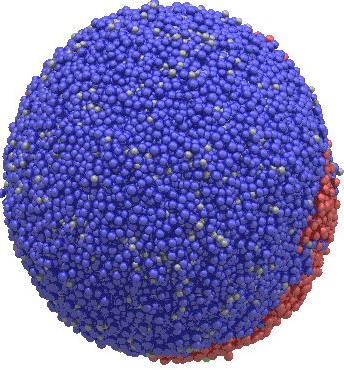
\includegraphics[width=1\textwidth]{result2/diag1b}
%\caption{time t=0)}
\label{}
\end{subfigure}\hspace*{-.5em}
%\centering
\begin{subfigure}[b]{.75\textwidth}
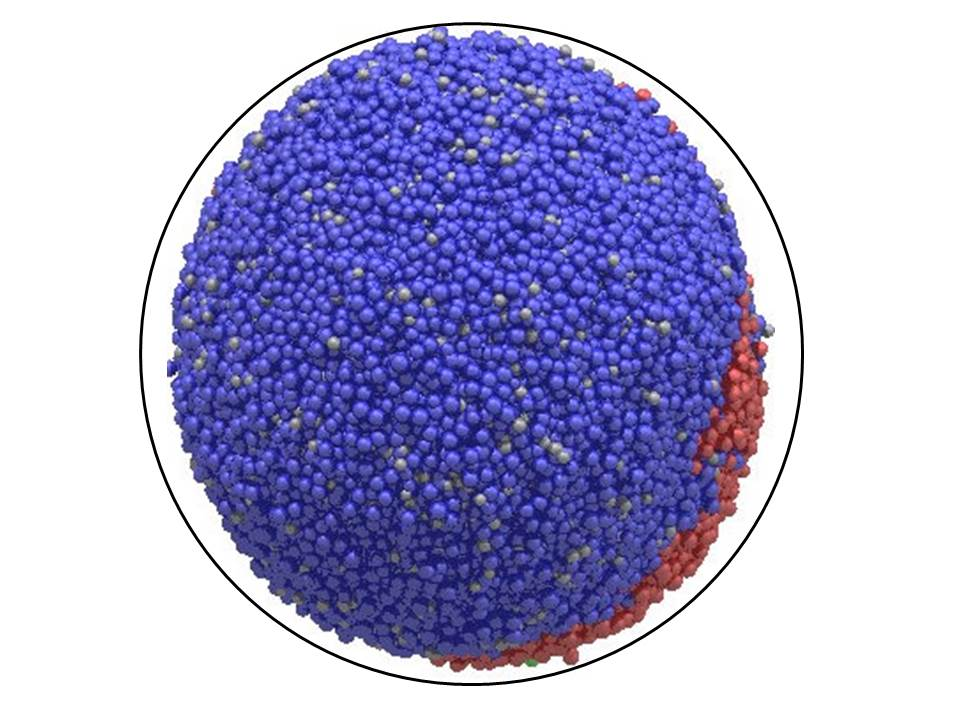
\includegraphics[width=1.02\textwidth]{result2/diag1bb}
%\caption{time t=100000}
%\label{diag2}
\end{subfigure}%\vspace*{-.1em}
\caption{Transformation of microscale particles to floc at the mesoscale for a particular time. Floc equivalent diameter is the diameter of the smallest sphere that circumscribes the outline of the projected floc.}\label{diag2}
\end{figure}

%\begin{figure}[!ht] 
%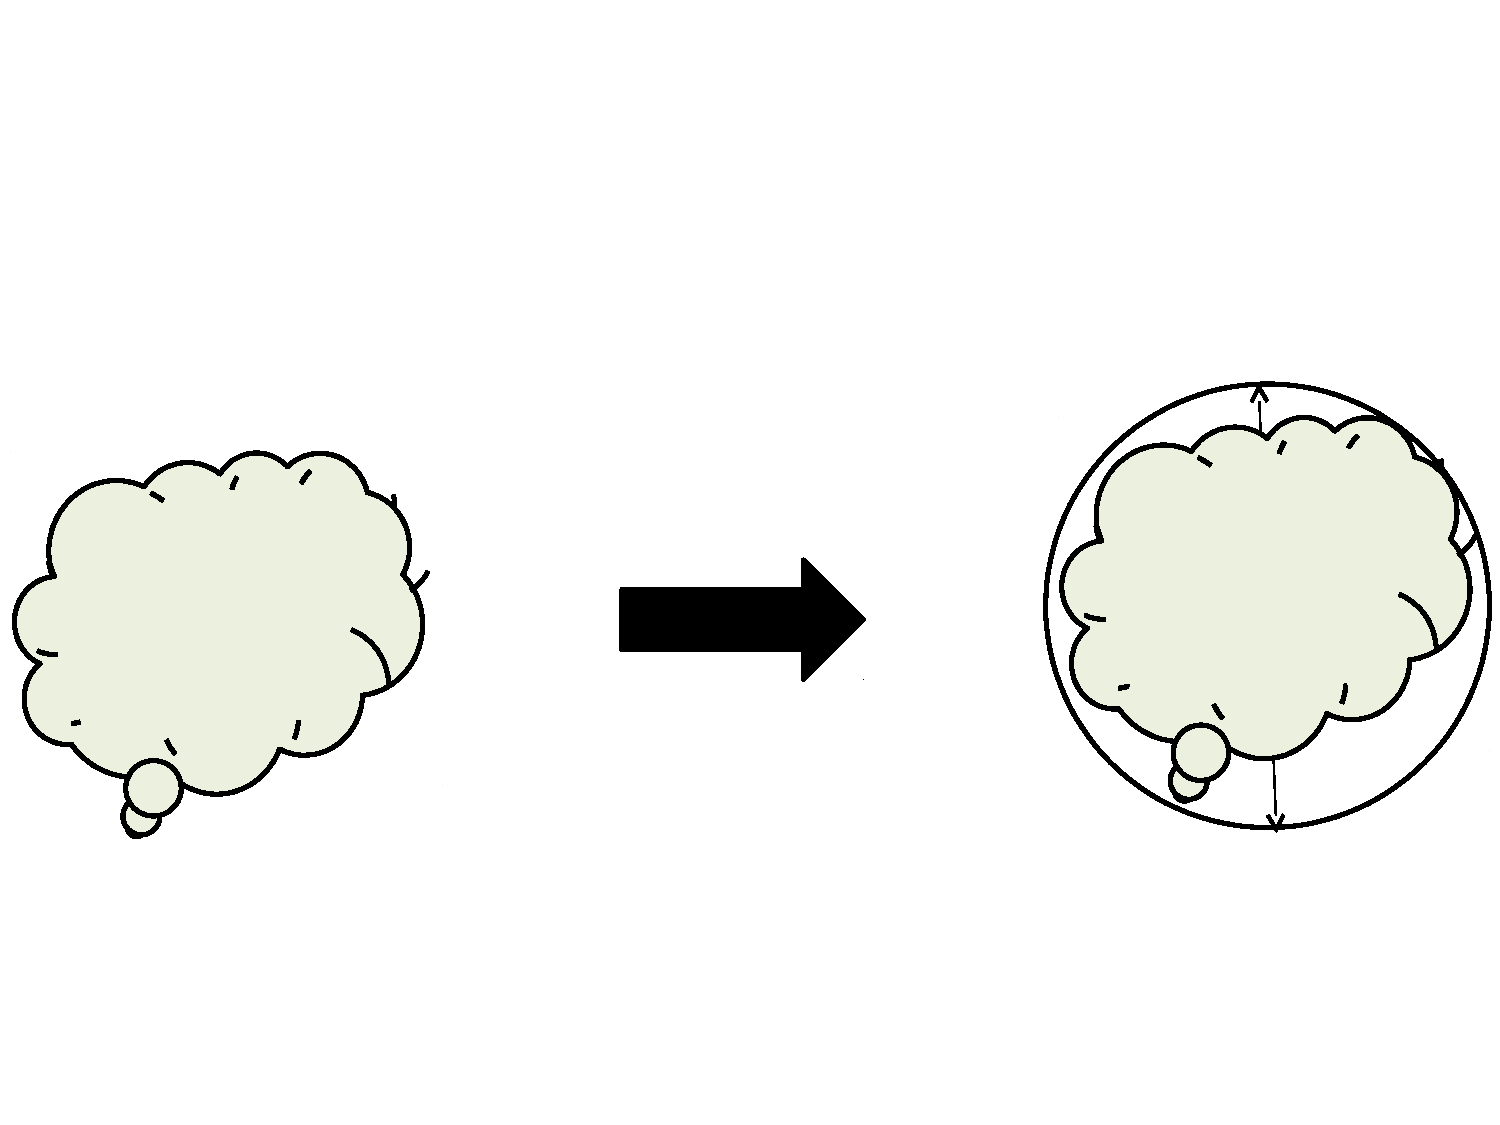
\includegraphics[width=1.1\textwidth]{diagram2}
%\caption[]{Transformation of microscale particles to floc at the mesoscale. Floc equivalent diameter is the diameter of the smallest sphere that circumscribes the outline of the projected floc.}\label{diag2}
%\end{figure}

\begin{figure}[!ht] 
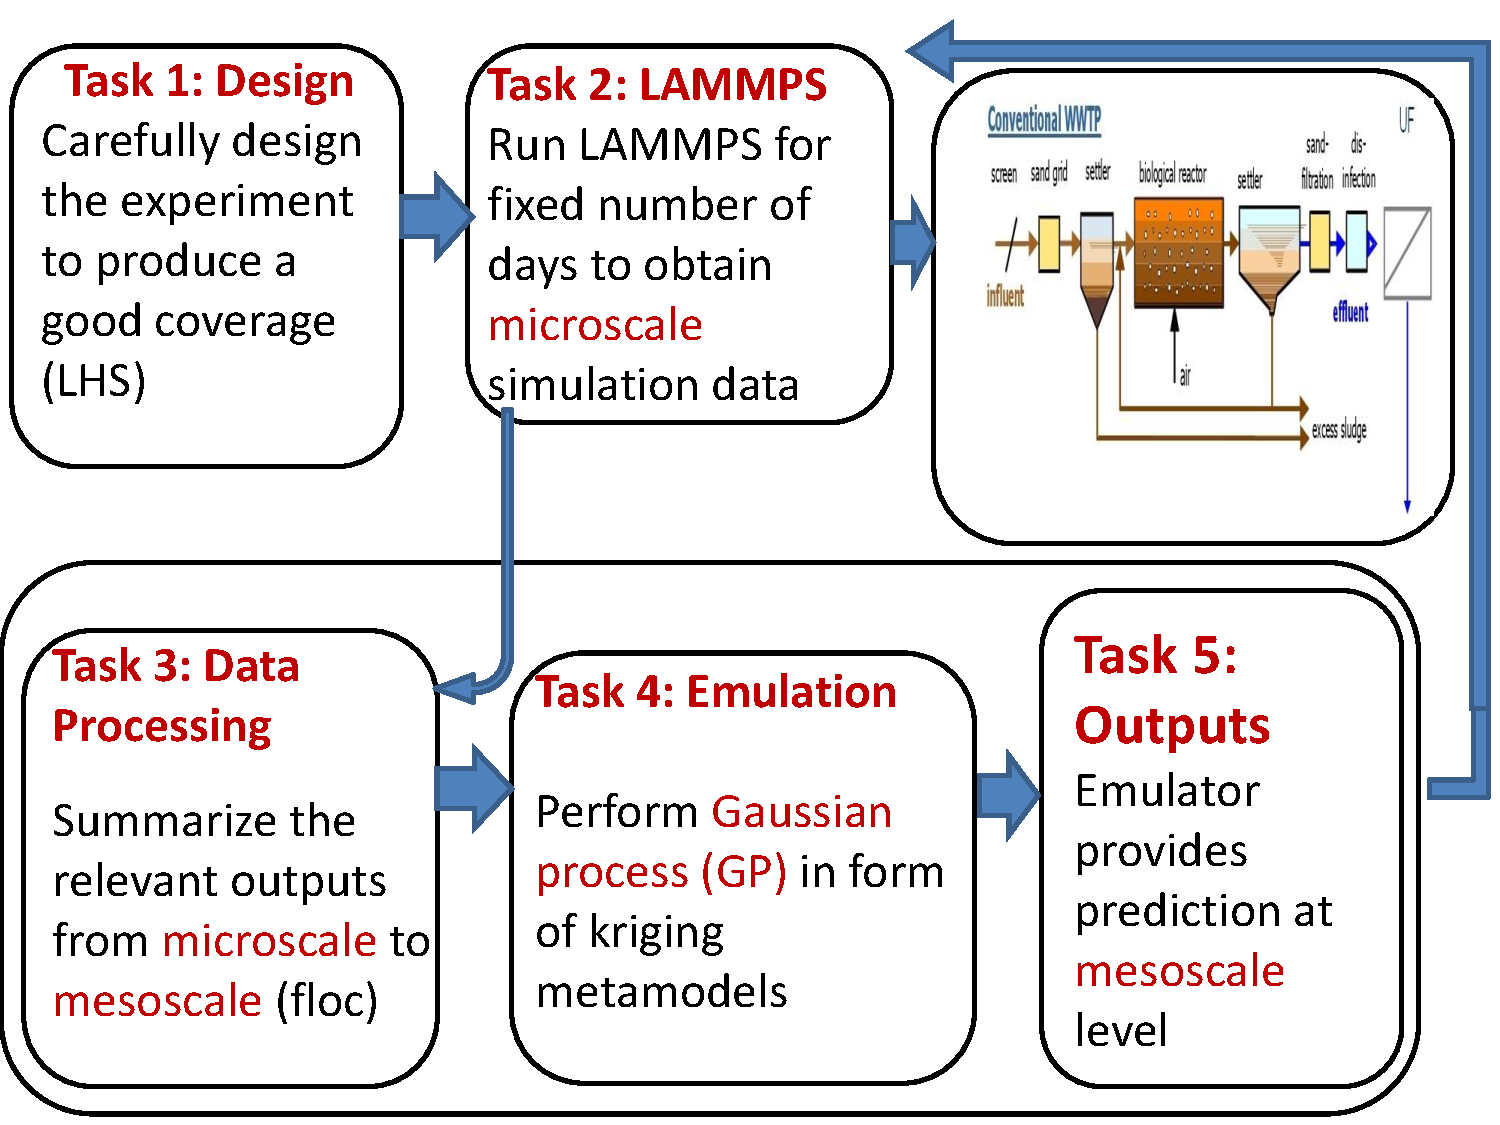
\includegraphics[width=1\textwidth]{result2/summ}
\caption[]{Schematic diagram showing key emulation stages}\label{diag2c}
\end{figure}

\newpage
\section{Methods}
 A Bayesian framework for emulation is almost always based on the assumption that a Gaussian process prior distribution can be specified for unknown parameters and hyperparameters.  Under a Bayesian perspective unknown parameters are treated as random variables. The given prior distribution can be updated from training data. Applying Bayes rule to this setting, a posterior distribution can be obtained. The posterior distribution is also a Gaussian process. We are implementing GP technique in form of kriging because of its wide applicability and flexibility. Another additional benefit of GP modelling is the quantification of the model uncertainty.

A major difficulty with GP modelling is the computational effort associated with dealing with large data, as computer time scales are of order $O(n^3)$ where $n$ is the number of observations. Several techniques have been adopted to overcome this computational problem. Earlier techniques are documented in \citet{q10} and \cite{q47}. GP emulation is based on the Bayesian technique and experimental design of computer experiments for predicting model outputs at test input point \citet{q7} and \citet{70}. A GP emulator assumes that a simulator output is an unknown function $g(.)$. We can then choose a prior distribution for $g(.)$ using the Bayesian approach and update this distribution, with some data obtained from the simulator runs.

\subsection{Kriging}
%Having obtained the simulation data by running the LAMMPS model as described in the previous section, we describe an alternative emulation approach for fitting LAMMPS output data. This approach involves using a kriging model, where the two stage techniques describe in previous section are combined as a single step. 
Kriging is a geostatistical technique for interpolating the value of an unknown random observation from data $\by(\bx)$ observed at known locations. Kriging models are also commonly used for building cheaper surrogate model of expensive computer codes \cite{pd1,pd2, pd3,pd6}. The two stage techniques describes in \citet{pd11} are combined as a single step. Here, $\by(\bx)$ can be decomposed into a mixture of deterministic (non-random trend) and a residual random variation. The trend could be modelled as a constant in ordinary/simple kriging or as an $n^{th}$ order polynomial in universal kriging. In this section, we shall discuss the universal kriging technique. The model formulation is given as
\begin{equation}\label{geneq2}
\by(\bx)= f(\bx) + \boldsymbol \varepsilon(\bx)
\end{equation}
where $\by(\bx)$ is the output of interest (eg floc equivalent diameter). The deterministic function $f(\bx)$ is the mean approximation of the expensive computer simulator (eg LAMMPS) and $f$ is a polynomial function. Under this assumption, $f(x)$ can be modelled as
\begin{equation}
f(\bx) = \sum_{j=1}^{p} \beta_j h_j(x) =\bH(x) \bbeta
\end{equation}
$\bbeta=[\beta_1,\ldots,\beta_p]$ is a $(p\times 1)$ vector of unknown regression coefficients and $\bH(x) = \Big[h_1(x), . . . , h_p(x)\Big]^T$ is a $(n\times p)$ matrix of regression functions,
$\varepsilon(\bx)$ is a stochastic Gaussian process with mean zero and characterize by its covariance function
$K=Cov(\varepsilon(\bx),\varepsilon(\bx)) = \sigma^2\bC(\bx,\bx')$, where $\sigma^2$ denotes the variance of $\varepsilon(\bx)$ also called process variance and $\bC$ is a $(n\times n)$ positive definite matrix of correlation between $\varepsilon(\bx)$'s at the experimental design points. We are assuming a univariate output and a deterministic computer model.

Similarly, $\bt(x^{new}) = \Big[Cor(x_1, x^{new}), \ldots,Cor(x_n, x^{new})\Big]^T$ for the $(n\times 1)$ vector of correlations between the $\varepsilon(\bx)$'s at the design points and new input points $x^{new}$. We use both Gaussian equation and exponential correlation functions, equations (\ref{gaus},\ref{expo}) \citet{pd4,pd18,pd19}.
%\begin{equation}
%\bC(x,x')=\Pi^{p}_{j=1}\exp^{-\balpha(x-x')^2}, 
%\end{equation}
%with a parameter $\balpha$. 
\begin{equation}\label{gaus}
\bC=\Big \{\exp(-(x-x')^T \boldsymbol \alpha (x-x')) \Big\},%\exp^{\Big[\sum \limits_{j=1}^{4}{-\boldsymbol \alpha_j(\bx_{j}-\bx^{\rm T}_{j})^2}\Big]}.
\end{equation}
\begin{equation}\label{expo}
\bC= \exp(-(x-x')/\alpha)
\end{equation}
where $\boldsymbol \alpha$ is the correlation hyperparameters to be estimated from the data.

The universal kriging predictor $\mu^{\bullet}(x^{new})$ of the value of $\by(x)$ at the new target point $x^{new}$ is the linear predictor
\begin{equation}
\mu^{\bullet}(x^{new})=\sum_{j=1}^n \lambda_j \by (x_j)=\lambda(x)^T\by,
\end{equation}
for the sample points $x_1, \ldots , x_n$, where the coefficients or weights $\lambda=(\lambda_1, \ldots, \lambda_n)^T$ are estimated by minimizing the variance of prediction error for each realizations of the random function $\by(x)$. The best linear unbiased predictor (BLUP) is computed by minimizing the mean squared error
\begin{equation}\label{mse}
MSE[\mu^{\bullet}(x^{new})]=E\Big[\lambda^T\by-\by(x^{new})\Big]^2,
\end{equation}
subject to the unbiasedness constraint $E\Big[\lambda^T(x)\by\Big] = E\Big[\by(x^{new})\Big]$. The mean squared error in equation (\ref{mse}) can be rewritten by substituting the value of $\by$ in equation (\ref{geneq2}), we thus have 
\begin{equation}
\sigma^2\Big[1 + c\lambda^T(x)\bC\lambda(x) - 2\lambda^T(x)\bt(x^{new})\Big],
\end{equation}
The unbiasedness constraint is now denoted as $H^T\lambda(x) = h(x)$. 
The optimal weights $\lambda^{*}_j$ in $\by(x^{new})$ is estimated by using Lagrange multipliers to constraining MSE minimization. The Lagrange multiplier is also use to solve system of equations in order to compute $p$ coefficients of $\lambda$.
Given the inverse of matrix $\bC$, then the best linear unbiased predictor for kriging model is given as
\begin{equation}\label{man}
\mu^{\bullet}_{uk}(x) = h^T(x)\hbbeta+ \bt^T(x)\bC^{-1}(\by -\bH\hbbeta)
\end{equation}
Similarly, the variance follows by substituting in the optimal value of $\lambda^*(x)$ in the MSE equation, we have
\begin{multline}\label{olu2b}%\tag{A.9}\label{olu2}
\begin{split}
\bK^{\bullet}_{uk}=\hat \sigma^2 \Big \{C(\bx,\bx') -\bt(\bx)^T\bC^{-1} \bt(\bx) + \\ \Big ( h(\bx)^T-\bt(\bx)^T\bC^{-1}\bt(\bx) \Big )
(\bH^T\bC^{-1}\bH)^{-1}\Big (h(\bx')^T-\bt(\bx')^T\bC^{-1}\bt(\bx') \Big )^T
\Big \}.
\end{split}
\end{multline}
See more details in \citep{pd4,pd5,pd20}.
%where $\hbbeta$ is given below.%= (\bH^T\bC^{-1}\bH)^{-1}\bH^T\bC^{-1}\by$.

The next problem is how to estimate the unknown parameters. We use a Maximum Likelihood Estimation (MLE) technique like many other authors \citep{pd5,pd28}, are being used as an estimator of the kriging model parameters because of its computational efficiency, $\theta=(\bbeta,\sigma^2,\boldmath \alpha)$. MLE is based on the assumption of Gaussian probability distribution. 
The likelihood of the model parameters is defined as the probability of the $n$ observations $\by= {y_1, …, y_n}$, given the model parameters such that 
\begin{equation}
L(\theta|\by)= \Pi_{j=1}^n p(\by_j|\theta).
\end{equation}
The expression for $L(\theta|\by)$ is given by equation below as
\begin{equation}\label{like*}
L(\boldsymbol \beta, \sigma^2, \boldsymbol{\alpha};\by)\propto \frac{|\bf C|)^{-\frac{1}{2}}}{{(2\pi\sigma^2)}^\frac{n}{2}}\exp \Big \{\frac{(\by-H\boldsymbol \beta)^T \bC^{-1}(\by-H\boldsymbol \beta)}{2\sigma^2}\Big\}
\end{equation}
where $\boldsymbol{\alpha}=[\alpha_1, \ldots, \alpha_n]$ is a vector of correlation lengths and $|\bC|$ is the determinant of correlation matrix $\bC$ and $K = \sigma^2\bC$.
By taking the derivative of the log-likelihood of equation (\ref{like*}) with
respect to $\bbeta$ and $\sigma^2$ and solving for zero, the estimates $\hbbeta$ and $\hat\sigma^2$ are given respectively as $\hbbeta=(\bH^T\bC^{-1}\bH)^{-1}\bH^T\bC^{-1}\by$ and $\hat{\sigma^2}=\frac{1}{n}\Big[\mathbf{(y-H\hat{\boldsymbol \beta})}^T\bf C^{-1}(\bf y-H\hat{\boldsymbol \beta})\Big]$. The alternative way of performing this computation under fully-Bayesian technique is to marginalise the conditional $\Big(f(.) | \by, \boldsymbol \beta, \sigma^2, \boldsymbol{\alpha}\Big)$ with respect to posteriors of $\boldsymbol \beta$ and $\sigma^2$. To estimate $\balpha$, we maximize over $\balpha$ and $\sigma^2$, the concentrated likelihood given below after plugging the values of $\hbbeta$ 
\begin{equation}
-2 log L(\hbbeta,\sigma^2, \balpha; \by) = n log(2\pi) +  log(|\bC|) + \Big \{(\by-\bH \hbbeta)^T \bC^{-1}(\by-\bH \hbbeta)\Big\}
\end{equation}
We observe that that both $\hat\sigma^2$ and $\bC$ depend upon the correlation parameter $\balpha$. The trend and covariance parameters $\theta$ can be computed quickly and very efficiently by using a global optimiser which is based on the extension of the efficient algorithm proposed in \citet{pd9} for likelihood maximization. Further details are provided in \citep{pd8}.

Because of the stochastic nature of the data we analyse in this paper, we briefly describe the extension of above derivation for the noisy observations, covariance $K=\sigma^2\bC$ is replaced by $ \sigma^2\bC+diag(\btau^2_1,\ldots,\btau^2_n)$ in equations (\ref{like*},\ref{olu2b},\ref{man}) respectively, where $\btau^2=\tau^2_1,\ldots,\tau^2_n$ are the noise variances. Kriging technique is equivalent to the Bayesian method describes in \citet{pd10} and \citet{q35}, if we assign improper uniform priors on the $\bbeta$. In other words, non-informative Bayesian analysis often leads to kriging predictor and variance and these estimators appear respectively as conditional mean and variance in equations (\ref{man} and \ref{olu2b}). The following is a summary of the calculations above.
\begin{itemize}
\item[{(i)}] Perform the kriging emulation of data $\by$. 
\item[{(ii)}] Given the posterior density of $\alpha$ as defined in equation (\ref{like3}) of Appendix 1, compute the MLE of $\balpha$, such that equation (\ref{like3}) is maximized.
\item[{(iii)}] Set $\bC= \bC(\bhalpha)$.
\item[{(iv)}] Compute estimate $\hbbeta=(\bH^T\bC^{-1}\bH)^{-1}\bH^T\bC^{-1}\by$
\item[{(v)}] Compute estimate $\widehat{\sigma^2}=\frac{1}{n}\Big[\mathbf{(y-H\hat{\boldsymbol \beta})}^T\bf C^{-1}(\bf y-H\hat{\boldsymbol \beta})\Big]$.
\item[{(vi)}] Compute posterior mean estimate $\mu^{\bullet}_{uk}(x)$ given in equation (\ref{man}).
\item[{(vii)}] Compute posterior variance estimate $\bK^{\bullet}_{uk}$ given in equation (\ref{olu2b}) above.
\end{itemize}

\subsection{Multivariate kriging}
Multivariate kriging extends kriging to $m$ observation types popularly called 'cokriging'. Cokriging has been widely
applied in various area especially in multifidelity surrogate models \citep{co3,co5} where there are array of $m$ levels of code usually from the expensive (accurate) to the less expensive (crude) simulators.

Suppose we have $m$ output levels of code $\bY(x)=(Y_1(x), \ldots, Y_m(x))$, %$x \elem R$
The $k^{th}$ output $y_k(x)$ is modelled as a Gaussian process $y_k(x) = Y_k(x)$. We use an autoregreesive ($AR$) model earlier proposed by \citet{co4} which is based on Markov property such that $Cov(Y_t(x), Y_{t-1}(x′)|Y_{t-1}(x)) = 0, x \neq x'$
and recently applied by \citet{co1}. The model formulation assumes
\begin{equation}\label{cok1}
Y_k(x) =\rho_{k-1}Y_{k-1}(x) + \delta_k(x)
\end{equation}
for $k\in (2,\ldots,m)$, $\delta_k(x)$ is a Gaussian process that models the bias between the output $k$ and the output $k-1$ adjusted and $\rho_{k-1}$ is the scaling factor between $Y_k$ and $Y_{k-1}$. The $\rho_{k-1}$ can be further treated as a linear regression function such that 
\begin{equation}
\rho_{k-1}(x) = g^T_{k-1}(x)\gamma_{k-1}
\end{equation}
and $g^T_{k-1}(x)$ is a vector of regression functions with covariance function of the form
$c_k(x, x′) = \sigma^2_k r_k(x - x′; \balpha_k),$
 where $\sigma^2_k$ is the variance of the Gaussian process and $\balpha_k$ are the correlation hyper parameters of correlation function $r_k$. 
In addition, since each of $Y_k(x)$ is a GP then the joint process ($Y_1(x), \ldots, Y_m(x)$) is a multivariate GP with mean
\begin{equation}
E[Y_k(x)|\sigma^2, \balpha, \bbeta, \gamma] = h′_k(x)^T \bbeta
\end{equation}
and covariance function
\begin{equation}
cov \Big[Y_k(x),Y_k(x')|\sigma^2, \balpha, \bB, \gamma_k \Big]=\sum_{k=1}^m \sigma^2_k \Big( \prod \limits_{i=k}^{k-1} \rho^2_i(x)\Big) r_k (x-x′;\balpha_k) 
\end{equation}

where $\sigma^2=(\sigma_1^2,\ldots,\sigma_k^2)$, $\balpha=(\balpha_1,\ldots,\balpha_k)$,  $\bB=(\bbeta_1,\ldots,\bbeta_k)$ and $\gamma=(\gamma_2,\ldots,\gamma_k)$,  
$$h'_k(x)^T=\Bigg( \Big( \prod \limits_{i=1}^{k-1} \rho_i(x)\Big) g^T_1(x), \Big( \prod \limits_{i=2}^{k-1} \rho_i(x)\Big) g^T_2(x), \ldots,\rho_{k-1} g^T_{k-1}(x),g^T_k(x) \Bigg).$$
$\bX_k$ is a design matrix and
$\Psi_k(\bX_k, \bX_{k'})$ is a $(n_k \times n_{k'})$ correlation matrix.
Unlike \citet{co1} and \citet{co2} that uses the Bayesian estimation technique, we introduce a likelihood maximization approach of \citet{co3} in this analysis.
Under $k=2$ setting, then equation \ref{cok1} can be rewritten as 
\begin{equation}
Y_2(x) =\rho Y_{1}(x) + \delta(x)
\end{equation}
where the design matrix is now defined as
\begin{equation}
\bX=\Big(\bX_1, \bX_2    \Big)^T=(\bx^{(1)}_1,\ldots,\bx^{(n_1)}_1,\bx^{(1)}_2,\ldots,\bx^{(n_2)}_2)^T
\end{equation}
such that
\begin{equation}
\bY=\Big(\bY_1(\bX_1), \bY_2(\bX_2)  \Big)^T=(Y_1(\bx_1^{(1)}),\ldots,Y_1(\bx_1^{(n_1)}),Y_1(\bx_2^{(1)}),\ldots,Y_1(\bx_2^{(n_2)}))^T.
\end{equation}
The conditional distribution of the output at a new target point $\bx^{new}$ under a universal cokriging formulation is given as
\begin{equation}
\Big[\by_2(\bx^{new})|\by=\by_1,(\bbeta_1,\bbeta_2,\rho),(\sigma_1^2,\sigma_2^2),(\balpha_1,\balpha_2)\Big] \sim N(\mu_{Y_2}(\bx^{new}),\bK(\bx^{new}))
\end{equation}
the mean and variance functions are given respectively as
\begin{equation}\label{}
\widehat\bmu_{\by_2}{(\bx)}= h^T(\bx)\hbB+ \bt^T(\bx)\bSigma^{-1}(\by -\bH\hbB)
\end{equation}
\begin{equation}\label{}
\widehat \bK_{\by_2}(x)=\hat\rho^2\hat \sigma_1^2+ \hat\sigma_r^2 - \bt^T(\bx)\bSigma^{-1}\bt(\bx),
\end{equation}
where 
\[ 
\bB=
\left(\begin{array}{cc}
\bbeta_1\\
\bbeta_2
\end{array} \right)
\quad \mbox{,}
\quad 
\by=
\begin{pmatrix}
y_1\\
y_2
\end{pmatrix}, 
\quad
h'=(\rho g_1^T(\bx),g_2^T(\bx)),
\]
\begin{equation}
t(\bx)=\rho \sigma_1^2 \Psi_1(\bx,\bX_1), \rho^2\sigma_1^2\Psi_1(\bx,\bX_2)+\sigma_r^2\Psi_r(\bx,\bX_2))^T,
\end{equation}

and covariance matrix given as
\[ \bSigma=
\left(\begin{array}{cc}
\sigma_{1}^2\Psi_1(\bX_1,\bX_1)   ~~~~~~~~~~~~~~~~~~~~ ~~ \rho\sigma_{1}^2\Psi_1(\bX_1,\bX_2)\\
\rho\sigma_{1}^2\Psi_1(\bX_2,\bX_1)  ~~~~~~ \Big(\rho^2\sigma_{1}^2\Psi_1(\bX_2,\bX_2) + \sigma_{r}^2\Psi_r(\bX_2,\bX_2)\Big)
\end{array} \right)\]

\[ \bH=
\left(
\begin{array}{cc}
g_1^T(x_1^{(1)}) ~~~~~~~~0\\
\vdots   ~~~~~~~~~~~~~~~~~~ \vdots       \\
g_1^T(x_{n_1}^{(1)}) ~~~~~~~~0  \\

\rho g_1^T(x_1^{(2)}) ~~~~~~~~g_2^T(x_1^{(2)})\\
\vdots   ~~~~~~~~~~~~~~~~~~ \vdots       \\
\rho g_1^T(x_{n_2}^{(2)}) ~~~~~~~~g_2^T(x_{n_2}^{(2)})
\end{array} 
\right)
 \quad = \quad
\begin{pmatrix}
F_1(\bX_1)~~~~~~~~~~0\\
\rho F_1(\bX_2) ~~~~~~~F_2(\bX_2)
\end{pmatrix}.
\]
The next problem is how to estimate the unknown parameters $(\bbeta_1,\bbeta_r,\rho,\sigma_1^2,\sigma_r^2,\balpha_1,\balpha_r)$. We use a maximum likelihood approach of \citet{co3} and \citet{co4}.
Firstly, we consider estimating the parameters $\theta_1=(\bbeta_1,\sigma_1^2,\balpha_1)$ and  $\theta_2=(\bbeta_r,\rho,\sigma_r^2,\balpha_r)$ differently because of the conditional independence that exists between the data $Y_1(x)$ and $Y_2(x)$. Therefore, we can maximize the log-likelihood given below to estimate $\theta_1$
\begin{equation}\label{cok3}
-\frac{n_1 log(\sigma_1^2)}{2} -  \frac{1}{2}log(|\Psi_1(\bX_1,\bX_1)|) - \frac{ \Big \{(\by_1-F_1 \bbeta_1)^T \Psi_1(\bX_1,\bX_1)^{-1}(\by_1-F_1 \bbeta_1)\Big\}}{2\sigma_1^2}
\end{equation}
where $|\Psi_1(\bX_1,\bX_1)|$ is the determinant of correlation matrix $\Psi_1(\bX_1,\bX_1)$, by taking the derivative of the equation (\ref{cok3}) with
respect to $\bbeta_1$ and $\sigma_1^2$ and solving for zero, the estimates $\hbbeta_1$ and $\hat\sigma_1^2$ are given respectively as
$$\hbbeta_1=(F_1^T \Psi_1(\bX_1,\bX_1) F_1)^{-1}F_1^T\Psi_1(\bX_1,\bX_1)^{-1}\by_1$$

and $\hat{\sigma_1^2}=\frac{1}{n_1} \Big[(\by_1-F_1\hbbeta_1)^T  \Psi_1(\bX_1,\bX_1)(\by_1-F_1\hbbeta_1)\Big]$.
The alternative way of performing this computation under fully-Bayesian technique of \citet{co1} and \citet{co2} is to marginalise the conditional $\Big(f(.) | \by_1, \bbeta_1, \sigma_1^2, \boldsymbol{\alpha_1}\Big)$ with respect to $\bbeta_1$ and $\sigma_1^2$. 
To estimate $\balpha_1$, we maximize over $\balpha_1$ the concentrated likelihood given below after plugging the values of $\hbbeta$ and $\hat{\sigma_1^2}$ in equation (\ref{cok3}) to give
\begin{equation}
-\frac{n_1 log( \hat \sigma_1^2)}{2} -  \frac{1}{2}log(|\Psi_1(\bX_1,\bX_1)|) 
\end{equation}

Secondly, we describe estimation of $\theta_2=(\bbeta_r,\rho,\sigma_r^2,\balpha_r)$. Let $\br=\by_2-\rho \by_1(\bX_2)$ and  $F=[F_2~~~~\rho \by_1(\bX_2)]$,
where $\by_1(\bX_2)$ are the collocated points of $\by_1$ and $\by_2$.
 Therefore, the log-likelihood of $\br|\by_2$ is given as
\begin{equation}\label{cok4}
-\frac{n_2}{2} log(\sigma_r^2) -  \frac{1}{2}log(|\Psi_r(\bX_2,\bX_2)|) - \frac{ \Big \{(\br-F \bbeta_r)^T \Psi_r(\bX_2,\bX_2)^{-1}(\br-F\bbeta_r)\Big\}}{2\sigma_r^2}
\end{equation}
$\hbbeta_r=(F^T \Psi_r(\bX_2,\bX_2) F)^{-1}F^T\Psi_r(\bX_2,\bX_2)^{-1}\br$, ~~~~~ $\hat{\sigma_r^2}=\frac{1}{n_2} \Big[(\br-F\hbbeta_r)^T  \Psi_r(\bX_2,\bX_2)(\br-F\hbbeta_r)\Big]$. Again, $\balpha_r$ and $\rho$ are estimated by maximized the restricted log-likelihood derived by substituting values $\hbbeta_r$ and $\hat{\sigma_r^2}$ in equation (\ref{cok4}). The trend and covariance parameters $\balpha_r$ and $\rho$ is computed quickly and very efficiently by using a global optimiser which is based on the extension of the efficient algorithm proposed in \citet{pd9} for likelihood maximization. Further details are provided in \citep{pd8}.

For $k=1$, our results is equivalent to universal kriging estimate. The derivation above can be extended to a case where $k>2$. The mean and variance can be estimated by using equation (\ref{cok1}). See futher detail in \citep{co4}.

Because of the stochastic nature of the data we analyse in this paper, we briefly describe the extension of above derivation for the noisy observations, covariance $K=\sigma^2\bC$ is replaced by $ \sigma^2\bC+diag(\btau^2_1,\ldots,\btau^2_n)$ in equations (\ref{like*},\ref{olu2b},\ref{man}) respectively, where $\btau^2=\tau^2_1,\ldots,\tau^2_n$ are the noise variances. Kriging technique is equivalent to the Bayesian method describes in \citet{pd10} and \citet{q35}, if we assign improper uniform priors on the $\bbeta$. In other words, non-informative Bayesian analysis often leads to kriging predictor and variance and these estimators appear respectively as conditional mean and variance in equations (\ref{man} and \ref{olu2b}). The following is a summary of the calculations above.



\[\bSigma=
\left(
\begin{array}{cc}
\sigma_1^2(\Psi_1 +I_{n_1\times n_1}\lambda_1) ~~~~~~~~~~~~~~~~~~~~~~~~~~~~~~~~~~~~~~~~\rho\sigma_1^2\Bigg[\Psi_{12}+\Big(0_{((n_1-n_2) \times n_2)}~~~I_{(n_1\times n_1)}\Big)^T\lambda_1\Bigg] 
\\
\rho\sigma_1^2\Bigg[\Psi_{21}+\Big(0_{(n_2 \times (n_1-n_2))}~~~I_{(n_1\times n_1)}\Big)\lambda_1\Bigg] ~~~~~~~~~\rho^2\sigma_1^2\Big(\Psi_{1'} +I_{n_2\times n_2}\lambda_1\Big) + \sigma_r^2\Big(\Psi_r +I_{n_2\times n_2}\lambda_2\Big)
\end{array} 
\right)
\]
where $\Psi_1=\Psi(\bX_1,\bX_1)$, ~~~ $\Psi_{12}=\Psi(\bX_1,\bX_2)=\Psi(\bX_2,\bX_1)$~~~ $\Psi_{1'}=\Psi(\bX_2,\bX_2)$~~~~~ and $\Psi_r=\Psi(\bX_2,\bX_2)$.
%$\rho^2\sigma_1^2\Big(\Psi_1 +I_{n_2\times n_2}\lambda_1\Big) + \sigma_r^2\Big(\Psi_r +I_{n_2\times n_2}\lambda_2\Big) $


%%%%%%%%%%%%%%%%%%%%%%%%%%%%%%%%%%
\begin{equation}\label{like*}
f(\bY)= \frac{|\bSigma_Y|^{-\frac{1}{2}}}{{(2\pi)}^\frac{mn}{2}}\exp \Big \{\frac{(\bY-\bH\bB)^T \bSigma_Y^{-1}(\bY-\bH\bB)}{2}\Big\}
\end{equation}

\[ \bSigma_Y=
\left(\begin{array}{ccc}
\bSigma_{11}~~\bSigma_{12}~~\ldots~~\bSigma_{1m}\\
\bSigma_{21}~~\bSigma_{22}~~\ldots~~\bSigma_{2m}\\
\vdots~~~~~~ \vdots ~~~\ddots~~~~\vdots \\
\bSigma_{m1}~~\bSigma_{m2}~~\ldots~~\bSigma_{mm} \end{array} \right)\]
where $\bSigma_{12}$ is the covariance between observations of type 1 and 2, $\bSigma_{11}$ is the 
univariate variance matrix. 
$$\hbB=(\bH^T\bSigma_Y^{-1}\bH)^{-1}\bH^T\bSigma_Y^{-1}\bY$$

\begin{equation}\label{man}
\bmu{(\bx)}= \bH^T(x)\hbB+ \bt^T(\bx)\hbSigma_Y^{-1}(\bY -\bH\hbB)
\end{equation}

\begin{multline}\label{olu2b}
\begin{split}
{\bK}= \Big \{\hbSigma_0 -\hbSigma_{0,mn}\hbSigma_Y^{-1}\hbSigma_{0,mn}  +  \bU (\bH^T\hbSigma_Y^{-1}\bH)^{-1}\bU^T\Big \}
\end{split}
\end{multline}


 $ \bU= I_n-\hbSigma_{0,mn}\hbSigma_Y^{-1}\bH$

 To estimate $\bSigma_Y$ which must be positive definite, we assume separable covariance model of the form $\bSigma_Y=\bSigma_0\bC$
 $\bSigma_0$ is the covariance matrix between different observation types and matrix $\bC$ is the input space covariance function. The joint likelihood of $\bSigma_Y$ and $\bB$ is obtained and maximized

%\item \alert{Univariate} - incorporate nugget terms in the form of empirical variance derived from replicates
%\item The extension for noisy observations, covariance $K=\sigma^2\bC$ is replaced by \alert{$ \sigma^2\bC+diag(\btau^2_1,\ldots,\btau^2_n)$}, where $\btau^2=\tau^2_1,\ldots,\tau^2_n$ are the noise variances
%\newline
%\item  \alert{Multivariate} - Follow  Kleijnen \& Beers(2005) approach of emulating a scale response
%\newline
%\item The scale response is derived by repeating the simulation $k$ times at each design point such that
%$\by'=\frac{\bar \by-\hat  f}{\mathbf{\sigma}^2/\sqrt{k}}$, where $\bar \by(x_i)=\frac{\sum \limits_{j=1}^k\by_{ij}}{k}$, $\sigma^2(x_i)=\frac{\sum \limits_{j=1}^{k}(\by_{ij}-\bar \by)^2}{k-1}$ and $\hat  f$ is estimate of main signal function
%\newline
%\item Apply kriging model to $\bY=[\by'_1,\ldots,\by'_m]$

%A Gaussian process model could not be applied directly to the stage 1 because of the computational difficulty in the sample size coupled with the large number of parameters to be estimated. GP scales cubically with the number of observations $O(N^3)$, which is not appropriate for our present data, even after averaging decadally and sampling from each scenario. The data matrix contains over 4.5 million observations. It is possible to use GP for residual interpolation. However, this approach still has a high computational cost, and it is necessary to reduce the spatial resolution and aggregate data to a country level in order to reduce the computational load. Our procedure is described below. 

%\subsection{Emulation procedure}
\subsection{Procedure for emulating LAMMPS outputs}
Here, we shall focus on the floc emulation and a single ouput from LAMMPS model. A single run of LAMMPS model consists of a simulation over many time steps which requires much computer workload and time taken. There are two different approaches to this problem. Firstly, we could emulate the simulator outputs (e.g., particles at the micro level) and use the emulator to link to the simulator at a mesoscale level for a floc. This approach is currently not practicable owing to a large number of simulation data involves, although it could be possible to perform some forms of data reduction. It is kikely that pattern decomposition might even complicate the upscaling problem. %The second approach that we adopt is to focus on the cluster of particles as a floc and emulate their interested properties directly. 

The second approach that we adopt is to focus on the cluster of particles as a floc because of a large number of data involve and emulate their interested properties like floc size. The floc is treated as a ball of a sphere, and we estimate the diameter of a sphere that circumscribes its boundary/outline. The center of the sphere will be equivalent to the center of mass of the component particles as shown Figure (\ref{diag2}). The detailed procedure of emulating the floc diameter will be described in this section and for biofilm in next section. In the further analysis, we will also emulate the center of the sphere to give spatial attributes to the floc characterization.

The LAMMPS model is a bit more complicated to emulate easily thus require a careful strategy.
Some of the major challenges of LAMMPS emulation are the nature of the outputs produced from the model itself that make it much difficult to emulate. The LAMMPS model is expensive to evaluate i.e slow and difficult to run for a large parameter space of interest, which limits the amount of information available for emulation. The model is stochastic in nature, this introduces much randomness in the data. The model is also dynamic in nature, the data are arraged as a sequence of outputs at different time points. Finally, the model produces high-dimensional and multiple outputs which make the emulation more computationally demanding than usual
Despite all these caveats, the good news is that there is a large knowledge base addressing these problems.

There is a limited number of literature that treat emulation of stochastic simulators. Earlier work of \citet{pd23} performs ordinary kriging emulation of detrended and standardized response $\by'$ from stochastic outputs. 
The scale response is derived by repeating the simulation $k$ times at each design point such that
$\by'=\frac{\bar \by-\hat  f}{\mathbf{\sigma}^2/\sqrt{k}}$, where $\bar \by(x_i)=\frac{\sum \limits_{j=1}^k\by_{ij}}{k}$, $\sigma^2(x_i)=\frac{\sum \limits_{j=1}^{k}(\by_{ij}-\bar \by)^2}{k-1}$ and $\hat  f$ is estimate of main signal function. This approach was extended by \citet{pd24} where an independent GP emulator is developed for both the mean response and stochastic (noise) variance.  A related approach was documented in \citet{pd22} and \citet{pd25} where an additional GP model is built to estimate the noise variance of the noise-free dataset.

In addition to develop a model for the mean response, \citet{pd21} also fit empirical log-transformed noise variance in an heteroscedastic GP modelling of a stochastic simulator. Similar to \citet{pd24} \citet{pd21}; \citet{pd26} focuses on the emulation and calibration of a stochastic computer model, implementing two independent Gaussian processes on the sample mean and log-transformed standard deviation of simulation outputs. The independent GP models use nugget parameters to account for sampling error in the data. 

Our initial treatment of the stochasticity in the model is to perform multiple runs and average the key outputs which are then taken as deterministic in nature. The second approach we use is to incorporate nugget terms in form empirical variance derived from the repeated simulation data.

\subsection{Dynamic emulation}
Due to the nature of output data from LAMMPS model, we consider using a dynamic emulation technique. Dynamic emulation models the evolution or trajectory of random variables over some time-steps \citep{pd12}. Emulation of time-series data or physical processes that evolve with time which implies that model output at time $t$ becomes an input to the model at time $t+1$. The model can be written as 
\begin{equation}\label{dyna3}
\by_t = f(\bx_t, \by_{t-1})
\end{equation}
Where $\by_{t-1}$ is the state vector at the previous time step for $t={1,\ldots,T}$, and $\bx_t$ are the inputs at time $t$ which includes the model parameters, forcing and initial conditions. There are two fundamental techniques for addressing dynamic emulation as discussed in \citep{pd12}. The multi-step and single-step emulations and there are about three different variants of the multi-step technique.

Firstly, under the multi-step emulation procedure, we can emulate a complete multi-step run of the computer model. One of the ways to proceed with this according to \citet{pd14} is to treat the problem as a multivariate output simulator and develop a multi-output emulator where the dimension of the output space is given as $T$. Closely related to this approach, is to build one single-output emulator that incorporates time as an additional input to the emulator such that $\by_t = f(\bx,t)$, where the training data for building emulator consists $nT$ data points. The limitation of this approach is that it is inefficient in practice because the dimension of the data becomes vast which introduces additional computational difficulty. 

The third variant is to emulate each time step, which produces an emulator that is specific to a particular time step, an approach that assumes independence between the time steps. This method was used in \citet{pd27} but is not suitable for our present data. Here, where are interested in the temporal correlations across the time steps, and specifically for using an emulator to scale up LAMMPS model outputs from an order of O($10^6$) particles to O($10^{13}$) particles, i.e., for making multiple-step ahead predictions. 

Under the single-step procedure, the method uses the simpler, single step simulator and use the emulator repeatedly to generate the full-time series of the resulting predictions up to the number of desired time points. This framework reduces the dimension of the problem. We implement both methods for emulation floc equivalent diameter. Although, the single-step emulation seems much appealing for our upscaling problem considering fact that we want to capture the complete behaviour of floc diameter over a number of time steps.
We describe the single-step procedure below.

\subsubsection{Single-step emulation}
We describe the single step function emulation here. We follow a similar procedure described in \citet{pd12,pd15}. Starting from initial run of the model at time $t_0$, we construct the single step emulator $\by_1 = f(\bx_1, \by_{0})$ using a GP regression in form of kriging. One of the usefulness of dynamic emulation is to make a multiple step ahead predictions using iterative technique to repeat one-step-ahead predictions until the desired number of points. We proceed sequentially, feeding back the entire output distribution from the GP model, such that at time step $t=1$, for input $(\bx_1,\by_0)$, we sample from the distribution of $f(\by_0,\bx_1)$, the model output is given as $$\tby^{(s)}_1 \sim N \Big(\mu^{\bullet}(\bx_1,\by_0), \bK^{\bullet}(\bx_1,\by_0)\Big).$$


For the next prediction at time $t=2$, the input data $\bx_2$ is augmented by complete distribution $\by^{(s)}_1$ such that $\bX_2=[(\bx_2,\tby_1)]^T$,  then we generate sample from the distribution of $f(\tby^{(s)}_1,\bx_2)$ and denote as $\tby^{(s)}_2 $, note that distribution of $\tby^{(s)}_2 $ is no longer normally distributed.
%then we have $$\tby^{(s)}_2 \sim N \Big(\mu^{\bullet}(x_2,\tby^{(s)}_1), \bK^{\bullet}(x_2,\tby^{(s)}_1)\Big).$$
This procedure is repeated until $T-1$ steps is reached. The construction of single-step emulator is summarized below:
\begin{itemize}
 \item[{(i)}] Subsample 300 points randomly from original 1000 points and formulate a single step emulator using equation (\ref{dyna3}) such that $\by_1=f(\bx,\by_0)$, where $\bx$ is the new design matrix for running the LAMMPS model for the single step function, $\bx$, as usual, include initial conditions and calibrated (constant) parameters while the corresponding output is the value of current state variable $\by_t$.

\item[{(ii)}] Perform the GP emulation in the form of kriging as described in previous chapter 2, where we use a quadratic mean and Matern covariance functions. Parameters $\theta=[\hbbeta, \hat{\sigma^2},\bhalpha]$ are estimated by MLE technique.

\item[{(iii)}] Compute the posterior distribution of $\Big(f(.)|\by,\hat\theta \Big)\sim N \Big(\mu^{\bullet}(x_0), \bK^{\bullet}(x_0)\Big)$ where $\mu^{\bullet}(x)$ and $\bK^{\bullet}(x)$ are defined in equations (\ref{man}, \ref{olu2b}) respectively.

\item[{(iv)}] Use the emulator to simulate from $\Big(f(.)|\by_1,\hat\theta\Big)$  to obtain $\tby^{(s)}_{1}$ and then iterate the next steps for $t=1,\ldots,T-1$ to give a full time series $\Big[\tby^{(s)}_1,\ldots,\tby^{(s)}_{T-1}\Big]$. 

\item[{(v)}] Derive a new training data by augmenting the original data with simulated time series and rebuild the single-step emulator with the new training data given below. 
\[ 
\left( \begin{array}{ccc}
\mbox{Original inputs}\\
~\vdots \\
(\by_0,\bx_1)\\
(\tby_1,\bx_2)\\
~~\vdots \\
(\tby_{T-1},\bx_T) \end{array} \right)
 = 
\left( \begin{array}{ccc}
\mbox{Original outputs}\\
~\vdots \\
\tby^{(s)}_1\\
\tby^{(s)}_2 \\
~\vdots \\
\tby^{(s)}_{T}\end{array} \right).
\] 
\item[{(vi)}] Simulate $\tby^{(s)}_{t+1}$ from conditional distribution $\Big(f(.)|\by_t,\hat\theta\Big)$.  
\item[{(vii)}] Repeat the entire process many times to obtain $\tbY^{N}=\Big[\tby^{(s)}_1,\ldots,\tby^{(s)}_{T-1}\Big]^N$, for $s=1,\ldots,N$, where $\tbY^{N}$ is a sample from the joint distribution of $[\by_1,\ldots,\by_{T-1}]$ given the emulator training data and initial conditions and $N$ is the number of Monte Carlo (MC) sample.
\end{itemize}

\subsubsection{Normal approximations to recursive iterations}
One of the limitations of above procedure is that it is highly prone to numerical problems associated with the inversion of the covariance matrix as training data is augmented. Moreover, an additional computational cost is often involved. There is a simple normal approximation to the above procedure that can prevent repeated use of single emulator thus avoiding the computational difficulties.
Here, we summarize the approximation technique according to \citet{pd12}. This new procedue is based on the assumption that augmentation of training data at each iteration step will have a relatively minimal effect provided that we use a large sample size for building our single-step emulator, in other words, additional data at each step could be discarded. In addition, since our training data for the single step emulator $\by_t = f(\bx,t)$ is modelled as a GP, thus makes it difficult to derive a joint distribution for $\by_1,\ldots,\by_T$ in a closed form, rather a normal approximation is proposed to estimate the marginal distribution of each $\by_t$ for $t=1,\ldots,T$. Suppose, the marginal distribution of $\by_t$ can be approximated as $\by_t \sim N\Big(\mu_t(.), \bK_t(.)\Big)$, where $\mu_1 =\mu^{\bullet}(x_1,y_0)$ and $\bK_1=\bK^{\bullet}\Big((x_1,y_0),(x_1,y_0)\Big)$, $\mu^{\bullet}(.)$ and $\bK^{\bullet}(.,.)$ are already defined in equations (\ref{man} and \ref{olu2b}) respecctively.

Then we have
\begin{equation}
\mu_{t+1}=E\Big(\mu^{\bullet}(\by_t, x_{t+1})|f(\by)\Big),
\end{equation}
\begin{equation}
\bK_{t+1}=E\Big(\bK^{\bullet}(x_{t+1},\by_t),(x_{t+1},\by_t)|f(\by)\Big) +var \Big(\mu^{\bullet}(\by_t, x_{t+1})|f(\by)\Big).
\end{equation}
 Now, we can then estimate the two quantities above using simulation from Monte Carlo sampling to repeatedly revise the mean and variance of the single step emulator.
\begin{equation}
\hat \mu_{t+1}=\frac{1}{N}\sum \limits_{s=1}^N\Big(\mu^{\bullet}(\tby^{(s)}_t, x_{t+1})|f(\by)\Big),
\end{equation}
\begin{equation}
\widehat \bK_{t+1}= \frac{1}{N}\sum \limits_{s=1}^N\Big(\bK^{\bullet}(x_{t+1},\tby^{(s)}_t),(x_{t+1},y_t)|f(\by)\Big) +\frac{1}{N}\sum \limits_{s=1}^N \Big(\mu^{\bullet}(\tby^{(s)}_t, x_{t+1})|f(\by)\Big)^2,
\end{equation}
where $\tby^{(s)}_t$ is a sample from $N\Big(\mu_t(.), \bK_t(.)\Big)$. This approximation technique is also related to procedure earlier described in \citet{pd17,pd29,pd30} where  GP is applied to a nonlinear dynamic systems to propagate uncertainty in an iterative multiple-step-ahead predictions.

\section{Results}

\subsection{Fractals}
Fractals are of rough or fragmented geometric shape that can be subdivided in parts, each
of which is (at least approximately) a reduced copy of the whole. The number, very often non-integer, often the only one measure of fractals. It measures the degree of fractal boundary fragmentation or irregularity over multiple scales \citet{co8}.
%%%
Fractal dimension of a floc is a measure of the complexity of its external shape \citep{co7}. It reflects the hydrodynamic environment that produces microbial aggregates. The fractal dimension can also be used to study the process of aggregation in wastewater treatment where the
characteristics of the aggregates play a crucial role to the performance, and operational stability \citet{co6}. It quantifies the particle morphology and particle density and settling velocity are a
function of the fractal dimensions.

Unlike \citet{co7} that uses the relationship between the object area and perimeter to calculate the fractal dimension, we used the ration of radius of agglomerates to the mean radius of the particles as given by the formula below
\begin{equation}
R_a=\sqrt \frac{\sum \limits_{i=1}^n m_i d_i^2}{\sum \limits_{i=1}^n m_i}
\end{equation} 
\begin{equation}
R_m=\sqrt \frac{\sum \limits_{i=1}^n r_i}{n}
\end{equation} 

\begin{equation}
F_D=\frac{log(R_a/R_m}{log(n)}
\end{equation} 
where $F_D$ is a fractal dimension. For Euclidean objects such as circles or squares, $F_D=1$, and for irregular particles such as flocs, $F_D<1$.

Span is another important property. The span factor gives an
indication of the distribution width
%i=10
%dat=dd[[i]]
%xs=dat[,3];ys=dat[,4]
%qx=quantile(xs,prob=c(.05,.95,.5))
%qy=quantile(ys,prob=c(.05,.95,.5))
%Xspan=qx[2]-qx[1]
%Yspan=qy[2]-qy[1]
%span=(Xspan+Yspan)/2
%%%%%%%%%%%%
Suppose at time step $t$, the LAMMPS output is written in the form 
\begin{equation}
\by_t=f(\bx_t,\by_{t-1})
\end{equation}
Where $\by_{t-1}$ the state vector at the previous time step, $\bx_t$ are the input at time $t$ which includes the model parameters, forcing and initial conditions as described earlier. We summarize the individual particle at microscale to a large (mesoscale) as a floc. We consider emulation of floc which is summarized by aggregating all the individual microbe at each time step. The number of particles $n$ at each time slice varies across the design points as stated before. The number of design points at each time step is $1000$ and $T=172$ in our simulation. The total floc mass at time $t$ is given as
\begin{equation}
M_t =\sum \limits^n_{k=1} m_{kt},
\end{equation} 
and center of mass $\tC$ for the floc aggregate in 3-dimension, for $X$ direction using equation 
\begin{equation}\label{com}
\tP_{x_t}=\frac{\sum \limits^n_{k=1} m_{kt} X_{kt}}{M_t},
\end{equation}
where $M_t$ is the total floc mass at time $t$ for all the species and $m_{kt}$'s are individual particle level mass. Replace $X_{kt}$ in equation (\ref{com}) with $Y_{kt}$ and $X_{kt}$ respectively to derive for other directions.

 There are two different ways to derive the floc equivalent diameter namely the volume and distance techniques. Under the distance approach, the diameter of the smallest circle that circumscribes the outer edge or sketch of the floc can be obtained by computing relative distances in $X-Y-Z$ positions of each of the particle from the center of mass of the floc aggregate. The sum of the maximum of this distances and radius of the particle with the largest distance will form the radius of the outer sphere as shown in Figure (\ref{diag2}). 

Suppose at time $t$, the distance in euclidean three-space between any two positions, say particle $p$ at position $P=(x_k,y_k,z_k)$ and floc center of mass at point $\tP=(x_0,y_0,z_0)$ is given as
\begin{equation}
 d_{k}=\sqrt{(x_{kt}-x_0)^2+(y_{kt}-y_0)^2+(z_{kt}-z_0)^2}, 
\end{equation}
\begin{equation}
d_{eqv}=2(\max{(d_{k})}+r_{k'}) ,
\end{equation}
where $r_{k'}$ is the radius of particle with largest distance and $x$, $y$ and $z$ are respective directions, $k=1,\ldots,n$. 
The second approach is to compute the total volume of the floc using the volume of each individual particle (particle is taken as a sphere).
\begin{equation}
d_{eqv}=\sum^n_{k=1} \sqrt[3]{\frac{6V_{kt}}{\pi}}
\end{equation}
where $V_{kt}$ volume of individual spherical particle $k$ at time $t$, $\pi$ is a constant and $d_{eqv}$ is the floc equivalent diameter. The volume technique under-estimates the value of equivalent diameter.

We apply the kriging model to train the data for floc equivalent diameter $d_{eqv}$ using a normal approximation technique of dynamic emulation. The output data for training the emulator are denoted as $\by=d_{eqv}$ and the corresponding input data are stored as a matrix .
Some results are given below.

\begin{figure}[!ht] 
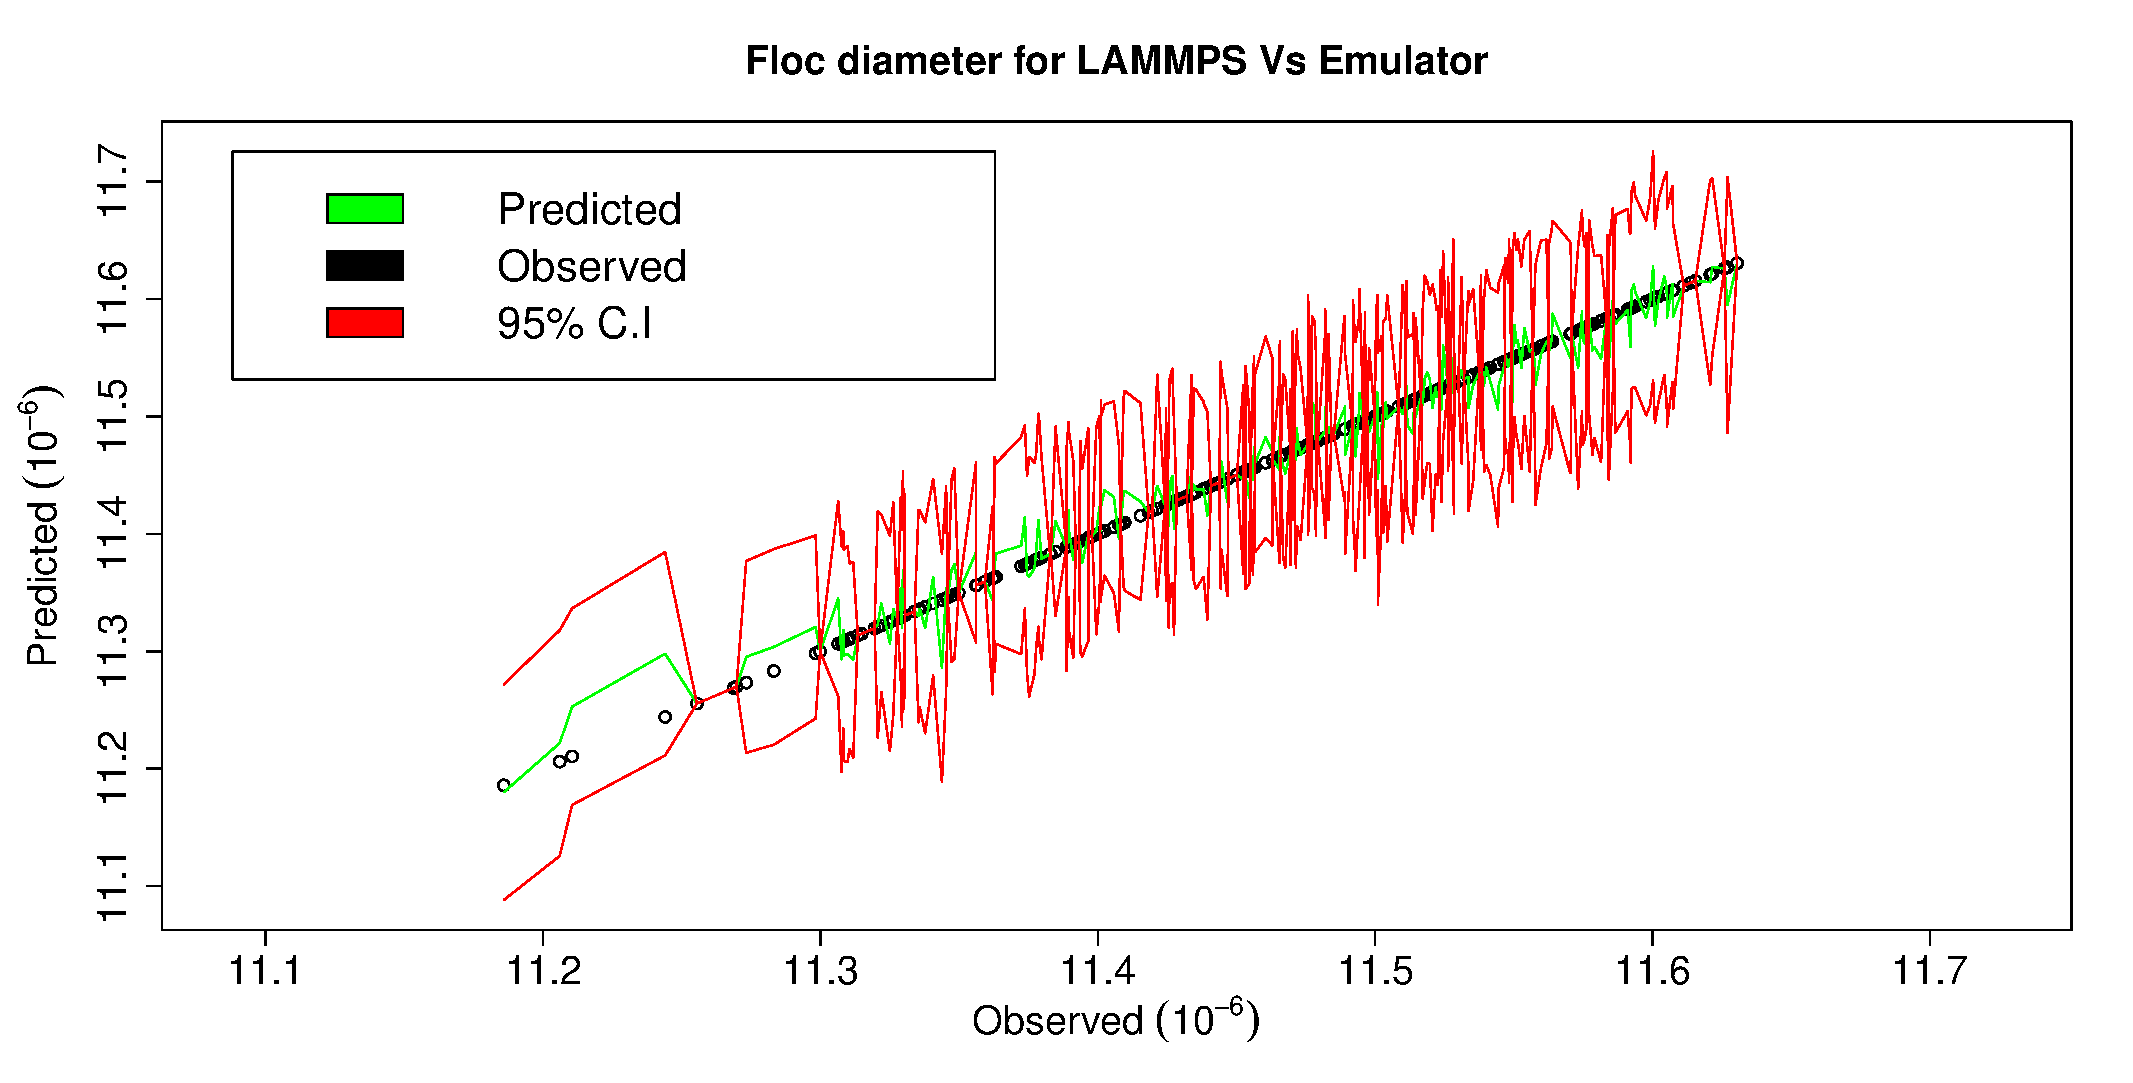
\includegraphics[width=1.1\textwidth]{result2/plot1}
\caption[]{Comparison between floc diameter for LAMMPS model and emulator with 95\% C.I}\label{diag2d}
\end{figure}

\begin{figure}[!ht] 
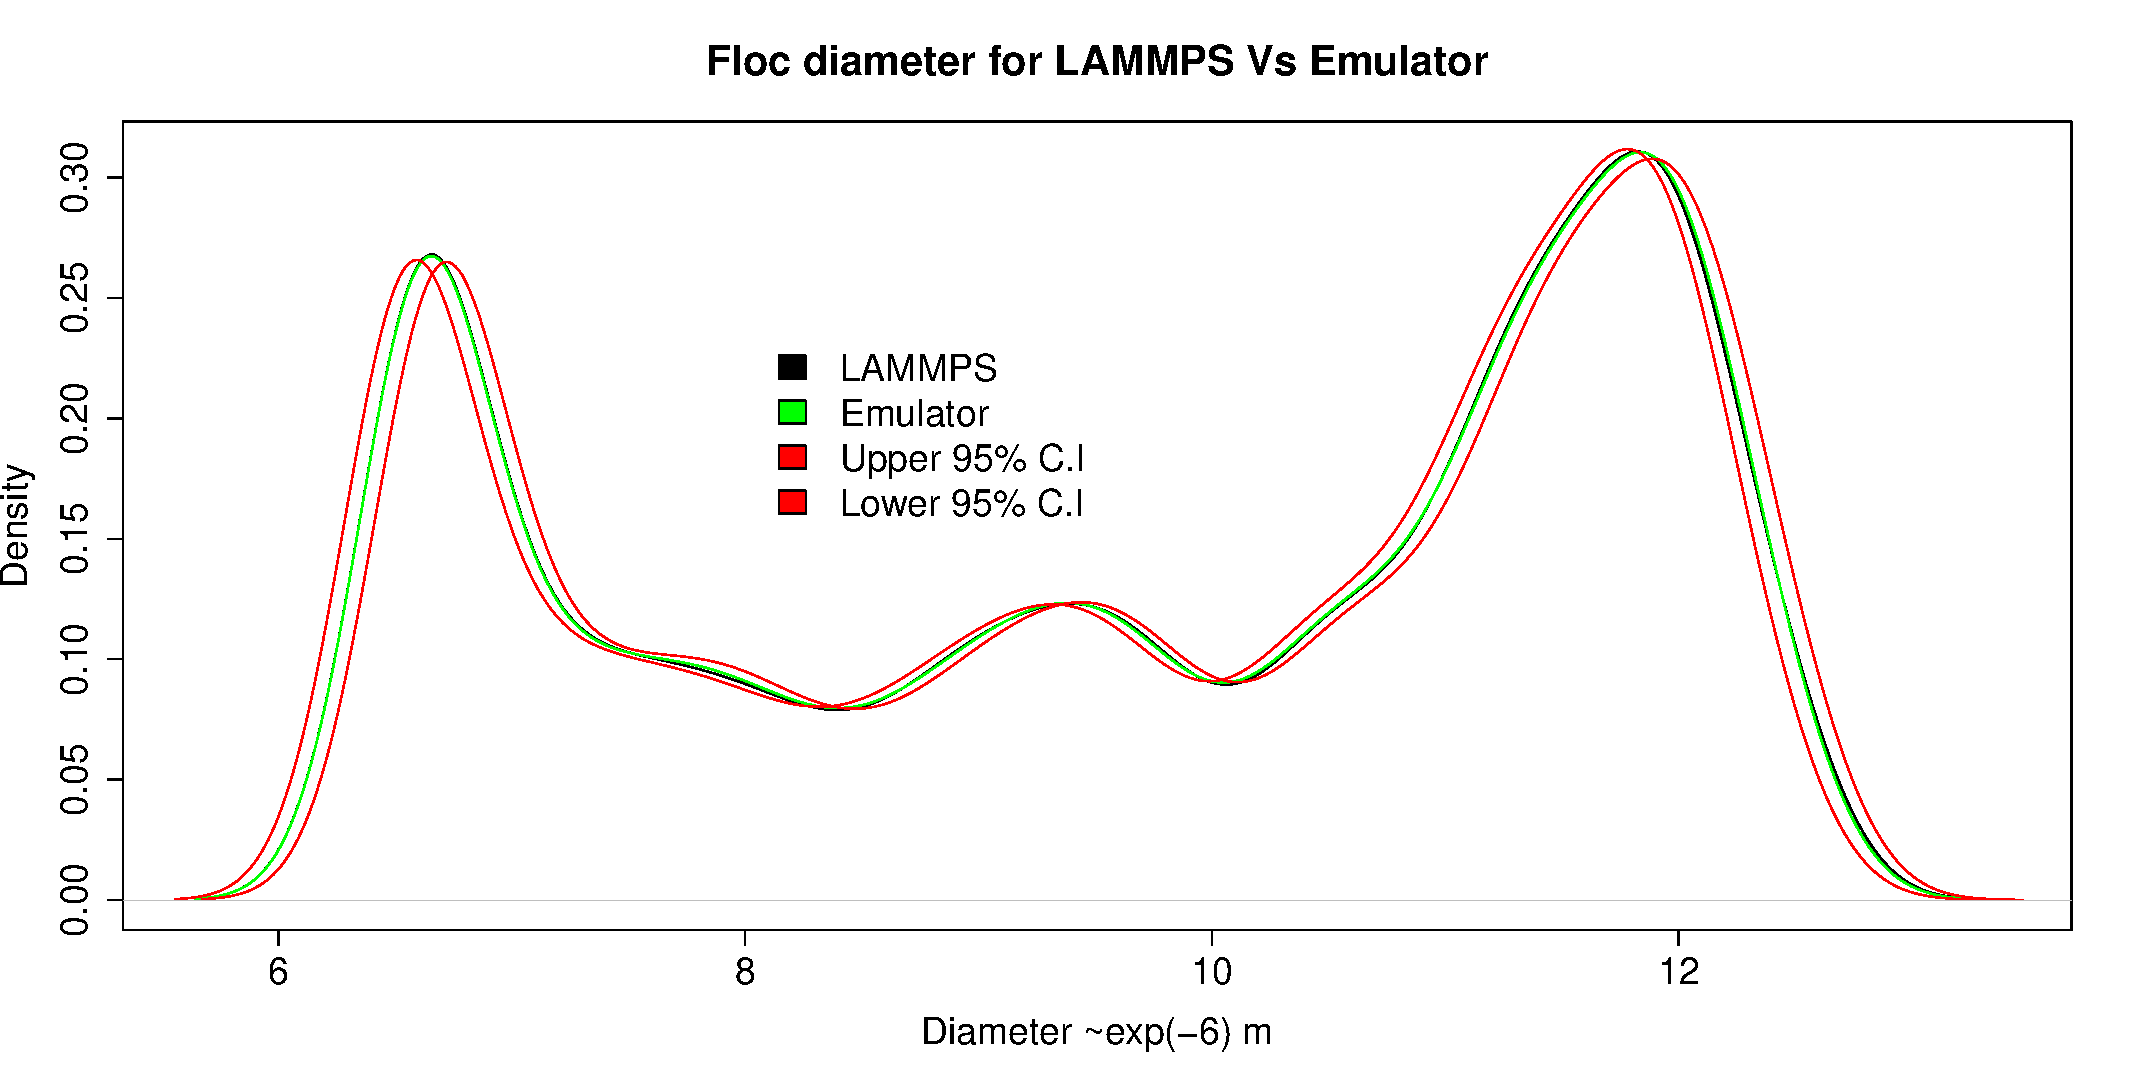
\includegraphics[width=1.1\textwidth]{result2/pdf}
\caption[]{Probability density function for LAMMPS model and emulator with 95\% C.I}\label{diag2e}
\end{figure}

\subsection{Emulator Performance}
\begin{itemize}
\item[(i)] It takes LAMMPS model between (13-24 hours) to obtain 2 days simulation ensembles on  8G  ram,  4-cores  Linux  machine.
\item[(ii)] Emulator gives results almost instantaneously (~2 minute).  
\item[(iii)] This is ~1100-fold increase in computational efficiency.
\end{itemize}


%\begin{itemize}
%\item[(i)] Biofilm /floc total mass at each time step
%\item[(ii)] Biofilm /floc equivalent diameter at each time step
%\item[(iii)] EPS total mass at each time step
%\item[(iv)] Total number of particles at each time step
%\item[(v)] The mass ratio of individual particle to the total biofilm /floc mass
%\item[(vi)] Distribution of floc/ biofilm diameter
%\item[(vii*)] Change in the nutrient environment of the floc (defer until the chemistry and hydrodynamics are coupled to the model).
%\item[(viii*)] Biofilm surface enlargement (still tricky; need to liaise with Prashant/Jaya)%\end{itemize}

\section{Biofilm emulation}
We describe emulation of biofilm in this section, we characterize the biofilm as shown in the Figure \ref{diag22} below. We apply the same procedure for emulating floc to the biofilm modelling.

\begin{figure}[!ht] 
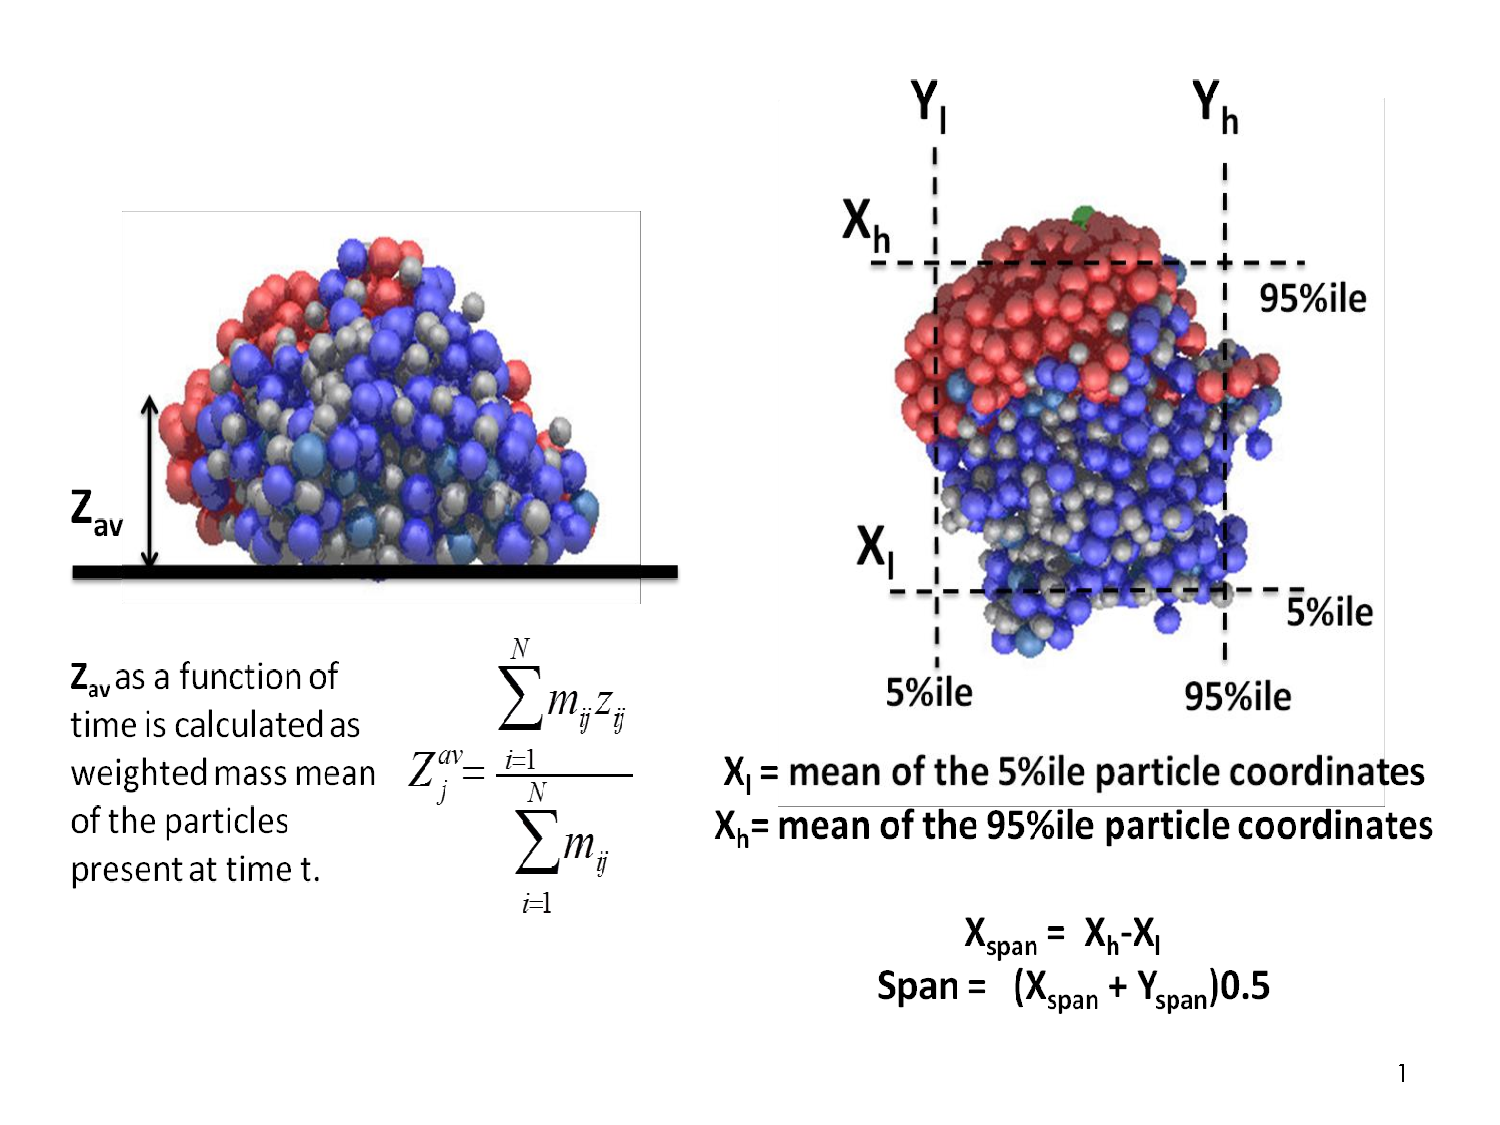
\includegraphics[width=1.1\textwidth]{result2/bio_char}
\caption[]{Biofilm characterization}\label{diag22}
\end{figure}

\section{Discussion}
%The reason for applying the GP on residual from model results instead of the simulation data. Our simulation data for both crops and climate are high-dimensional gridded global data that cannot be modelled directly by GP. Several approximation techniques have been developed to handle multi-dimensional data. For instance, a low-rank approximation of the Gram matrix was described in \cite{q10,q11}. The use of subsets of regressors and subsets of data to reduce the computational burden of the GP inversion for a large data matrix was investigated by \cite{q12,q13,q14}. The following studies used Bayesian techniques for emulating high-dimensional data \cite{q28,q29,q22,q23,qq}. A good emulator must be as fast as possible to allow for relatively quick evaluation of many scenarios which are not feasible with these techniques. Therefore, the Bayesian procedures used in the studies mentioned above cannot be directly applied to handle large dimensional and high-resolution crop data in this study. 

%Another way to resolve our problem is to treat each spatial point as a GP and then emulate each grid cell individually a technique implemented in \cite{q62} and \cite{q64}. However, this option is intractable since we have 59199 grid points meaning that about 236,796 emulators have to be constructed and validated for the four crops we are emulating.

\section{Conclusion}
In this paper, we have demonstrated a means of making inference about the parameters of the emulator using a GP regression that is based upon kriging. We have presented a simple statistical method for emulating the underlying physical dynamics of response of potential floc diameter. %We use combinations of stepwise regression, PCA and GP methods to emulate major crop-yield as a linear function of seasonal climate variables and other relevant variables. Aggregated country average of actual yield change is calculated by combining yields simulated by LPJmL for both rainfed and irrigated. We consider eight time-slices averaged over ten years, baseline corresponding to the average (2005-2014). 

In modelling the residual micro scale particle, we reduced the complexity of the computation by aggregating spatially from a fine to a more coarse resolution as a floc. We assume that the aggregation will reduce the complexity and structure of the global trend component of the emulator. %We have already seen from the residual plots that some variations have not been accounted for by the stepwise regression model. It is important to reduce the dimensionality of data for tractable application of GP modelling. 
 
%\begin{acknowledgements}
%If you'd like to thank anyone, place your comments here
%and remove the percent signs.
%\end{acknowledgements}

% BibTeX users please use one of
%\bibliographystyle{spbasic}      % basic style, author-year citations
%\bibliographystyle{spmpsci}      % mathematics and physical sciences
%\bibliographystyle{spphys}       % APS-like style for physics
%\bibliography{}   % name your BibTeX data base

% Non-BibTeX users please use
%\begin{thebibliography}{}
%\end{thebibliography}


%\begin{thebibliography}{94}
%\cleardoublepage
%\phantomsection
%\bibliographystyle{plain}


\begin{thebibliography}{94}
%\cleardoublepage
%\phantomsection
\bibliographystyle{plain}
\bibitem[Currin et al.(1991)]{pd1} Currin, C., Mitchell, T.J., Morris, M.D., and Ylvisaker, D. (1991). Bayesian Prediction of Deterministic Functions, With Applications to the Design and Analysis of Computer Experiments. {\it Journal of the American Statistical Association}, $86(416), 953-963$. 

\bibitem[Martin \& Simpson(2004)]{pd2} Martin, J. D., \& Simpson, T. W. (2004). On the use of kriging models to approximate deterministic computer models. {\it In ASME 2004 International Design Engineering Technical Conferences and Computers and Information in Engineering Conference}, $481-492$.

\bibitem[Osio et al.(1996)]{pd3} Osio, I.G. and Amon, C.H. (1996). An Engineering Design Methodology with Multistage Bayesian Surrogate and Optimal Sampling. {\it Research in Engineering Design}, $8(4), 189-206$.

\bibitem[Sacks et al.(1989)]{pd4} Sacks, J., Welch, W., Mitchell, T., Wynn, H. (1998). Design and analysis of computer experiments. {\it Statistical Science}, $4(4), 409-435$.

\bibitem[Santner et al.(2003)]{pd5} Santner, T., Williams, B., Notz, W. (2003). The Design and Analysis of Computer Experiments. Springer.

\bibitem[Li \& Sudjianto(2005)]{pd6} Li, R., \& Sudjianto, A. (2005). Analysis of computer experiments using penalized likelihood in gaussian kriging models. {\it Technometrics}, $47(2), 111-120$.

\bibitem[Andrianakis \& Challenor(2009)]{pd7} Andrianakis, Y., \& Challenor, P. G. (2009). Parameter estimation and prediction using gaussian processes. {\it Technical report}, MUCM Technical report 09/05, University of Southampton.

\bibitem[Roustant et al.(2012)]{pd8} Roustant, O., Ginsbourger, D., \& Deville, Y. (2012). DiceKriging, DiceOptim: Two R packages for the analysis of computer experiments by kriging-based metamodeling and optimization.

\bibitem[Park \& Baek(2001)]{pd9} Park J.S., \& Baek, J. (2001). Efficient Computation of Maximum Likelihood Estimators in a
Spatial Linear Model with Power Exponential Covariogram. {\it Computer Geosciences}, $27, 1-7$.

\bibitem[Hankin(2005)]{pd10} Hankin, R. K. (2005). Introducing BACCO, an R package for Bayesian analysis of computer code output. {\it Journal of Statistical Software}, $14(16), 1-21$.

\bibitem[O'Hagan(2006)]{pd11} O'Hagan, A. (2006). Bayesian Analysis of Computer Code Outputs: A Tutorial. {\it Reliability Engineering and System Safety}, $91, 1290-1300$.

\bibitem[Conti et al.(2009)]{pd12} Conti, S., Gosling, J. P., Oakley, J. E., \& O'hagan, A. (2009). Gaussian process emulation of dynamic computer codes. {\it Biometrika}, asp028.

%\bibitem[Conti {\em et al}.(2004)]{pd13} Conti, S., Anderson, C. W., Kennedy, M. C., \& O’Hagan, A. (2004). A Bayesian analysis of complex dynamic computer models. {\it In Proc. of the 4th International Conference on Sensitivity Analysis of Model Output}.

\bibitem[Conti {\em et al}.(2010)]{pd14} Conti, S., \& O’Hagan, A. (2010). Bayesian emulation of complex multi-output and dynamic computer models. {\it Journal of statistical planning and inference}, $140(3), 640-651$.

\bibitem[Bhattacharya(2007)]{pd15} Bhattacharya, S. (2007). A simulation approach to Bayesian emulation of complex dynamic computer models. {i\t Bayesian Analysis}, $2(4), 783-815$.

%\bibitem[Kennedy {\em et al}.(2001)]{pd16} Kennedy, M.C., \& O'Hagan, A. (2001). Bayesian calibration of computer models. {\it Journal of the Royal Statistical Society}. Series B, Statistical Methodology, $425-464$.

\bibitem[Azman \& Kocijan (2005)]{pd17} Azman, K., \& Kocijan, J. (2005). Comprising prior knowledge in dynamic gaussian process models. {\it In Proceedings of the International Conference on Computer Systems and Technologies-CompSysTech}, Vol. 16(17.6).

\bibitem[Kleijnen(2009)]{pd18} Kleijnen, J. P. (2009). Kriging metamodeling in simulation: A review. {\it European Journal of Operational Research}, $192(3), 707-716$.

\bibitem[Kleijnen \& Simpson(2005)]{pd19} Martin, J. D., \& Simpson, T. W. (2005). Use of kriging models to approximate deterministic computer models. {\it AIAA journal}, $43(4), 853-863$.

\bibitem[Kleijnen \& Mehdad(2014)]{pd20} Kleijnen, J. P., \& Mehdad, E. (2014). Multivariate versus univariate kriging metamodels for multi-response simulation models. {\it European Journal of Operational Research}, $236(2), 573-582$.

\bibitem[Boukouvalas {\em et al}.(2009)]{pd21} Kleijnen, J. P. (2009) Boukouvalas, A., Cornford, D., \& Singer, A. (2009). Managing uncertainty in complex stochastic models: {\it Design and emulation of a rabies model. In 6th St. Petersburg Workshop on Simulation}, (pp. 839-841).

\bibitem[Kersting {\em et al}.(2007)]{pd22} Kersting, K., Plagemann, C., Pfaff, P., \& Burgard, W. (2007). Most likely heteroscedastic Gaussian process regression. {\it In Proceedings of the 24th international conference on Machine learning}, (pp. 393-400). ACM.

\bibitem[Kleijnen \& Beers(2005)]{pd23} Kleijnen, J.P., \& Van Beers, W.C. (2005). Robustness of kriging when interpolating in random simulation with heterogeneous variances: Some experiments. {\it European Journal of Operational Research}, $165(3), 826-834$.

\bibitem[Bates {\em et al}.(2006)]{pd24} Bates, R. A., Kenett, R. S., Steinberg, D. M., \& Wynn, H. P. (2006). Achieving robust design from computer simulations. {\it Quality Technology and Quantitative Management}, $3(2), 161-177$.

\bibitem[Bates {\em et al}.(1997)]{pd25} Goldberg, P. W., Williams, C. K., \& Bishop, C. M. (1997). Regression with input-dependent noise: A Gaussian process treatment. {\it Advances in neural information processing systems}, $10, 493-499$.

\bibitem[Henderson {\em et al}.(2012)]{pd26} Henderson, D. A., Boys, R. J., Krishnan, K. J., Lawless, C., \& Wilkinson, D. J. (2012). Bayesian emulation and calibration of a stochastic computer model of mitochondrial DNA deletions in substantia nigra neurons. {\it Journal of the American Statistical Association}.

\bibitem[Boukouvalas {\em et al}.(2014)]{pd27} Boukouvalas, A., Sykes, P., Cornford, D., \& Maruri-Aguilar, H. (2014). Bayesian precalibration of a large stochastic microsimulation model. {\it Intelligent Transportation Systems, IEEE Transactions on}, $15(3), 1337-1347$.

\bibitem[Kleijnen \& Mehdad(2012)]{pd28} Kleijnen, J., \& Mehdad, E. (2012). Kriging in multi-response simulation, including a Monte Carlo laboratory. {CentER Discussion Papers Series}, (2012-039).

\bibitem[Jarvis {\em et al}.(2005)]{l3} Jarvis, P., Jefferson, B., \& Parsons, S. A. (2005). Measuring floc structural characteristics. {\it Reviews in Environmental Science and Bio/Technology}, $4(1-2), 1-18$.

\bibitem[Frazer {\em et al}.(2013)]{l4}  Fraser, C. E., McIntyre, N., Jackson, B. M., \& Wheater, H. S. (2013). Upscaling hydrological processes and land management change impacts using a metamodeling procedure. {\it Water Resources Research}, $49(9), 5817-5833$.

 \bibitem[Wheater {\em et al}.(2008)]{l8} Wheater, H.S., B. Reynolds, N. McIntyre, M. Marshall, B. Jackson, Z. Frogbrook, I. Solloway, O. J. Francis, and J. Chell (2008). Impacts of upland land management on flood risk: Multi-scale modelling methodology and results from the Pontbren experiment, {\it FRMRC Res. Rep. UR}, 16, 163 pp., Imp. Coll. \& CEH Bangor, London, U.K.

 \bibitem[Van {\em et al}.(2009)]{l9} Van Oijen, M., Thomson, A., \& Ewert, F. (2009). Spatial upscaling of process-based vegetation models: An overview of common methods and a case-study for the UK. Methods, 1(3).
 
\bibitem[Ofiteru {\em et al}.(2014)]{l11} Ofiteru, I. D., Bellucci, M., Picioreanu, C., Lavric, V., \& Curtis, T. P. (2014). Multi-scale modelling of bioreactor–separator system for wastewater treatment with two-dimensional activated sludge floc dynamics. {\it Water research}, $50, 382-395$.

%\bibitem[Hankin(2005)]{pd32} Hankin, R. K. (2005). Introducing BACCO, an R package for Bayesian analysis of computer code output. {\it Journal of Statistical Software}, $14(16), 1-21$.

%%%%%%%%%%%%%%%%%




\bibitem[Higdon {\em et al}.(2008)]{q23} Higdon, D., Gattiker, J., Williams, B. \& Rightley, M. (2008). Computer model calibration using high-dimensional output. {\it Journal of the American Statistical Association}, $103, 570-583$.


\bibitem[Kennedy {\em et al}.(2001)]{45} Kennedy, M.C. \& O'Hagan, A. (2001). Bayesian calibration of computer models. {\it Journal of Royal Statistical Society}, series B, $63(3), 425-464$.

\bibitem[Kennedy {\em et al}.(2006)]{q17} Kennedy, M. C., Anderson, C. W., Conti, S., and O'Hagan, A. (2006). Case studies in Gaussian process modelling of computer codes. {\it Reliability Engineering \& System Safety}, $91, 1301-1309$.

%\bibitem[Kennedy {\em et al}.(2008)]{46} Kennedy, M.C. {\em et al}. (2008). Quantifying uncertainty in the biospheric carbon flux for England and Wales. {\it Journal of the Royal Statistical Society}, Series B, $171, 109-135$.




\bibitem[Oakley(1999)]{q35} Oakley, J. (1999). Bayesian Uncertainty Analysis For Complex Computer Codes. Ph.D. thesis, University of Sheffield.

\bibitem[Oakley \& O'Hagan(2002)]{60} Oakley, J. and O'Hagan, A. (2002). Bayesian inference for the uncertainty distribution of computer model outputs. {\it Biometrika}, $89, 769-784$.

\bibitem[Oakley \& O'Hagan(2004)]{q5} Oakley, J. E. and O'Hagan, A. (2004). Probabilistic sensitivity analysis of complex models: a Bayesian approach.{\it Journal of Royal Statistical Society}, $66B, 751-769$.


\bibitem[Oyebamiji {\em et al}.(2015)]{qwole} Oyebamiji, O.K., Edwards, N.R., Holden, P.B., Garthwaite, P.B., Schaphoff, S., and Gerten, D. (2015). Emulating global climate change impacts on crop yields. {\it Statistical Modelling}, 1471082X14568248.

%\bibitem[O'Hagan(2006)]{l5} O'Hagan, A. (2006). Bayesian Analysis of Computer Code Outputs: A Tutorial. {\it Reliability Engineering and System Safety}, $91, 1290-1300$.

\bibitem[Higdon {\em et al}.(2008)]{l6} Higdon, D., Gattiker, J., Williams, B. \& Rightley, M. (2008). Computer model calibration using high-dimensional output. {\it Journal of the American Statistical Association}, $103, 570-583$.

\bibitem[Quinonero-Candela \& Rasmussen(2005)]{q47} Quinonero-Candela, J., \& Rasmussen, C. E. (2005). A unifying view of sparse approximate Gaussian process regression. {\it The Journal of Machine Learning Research}, $6, 1939-1959$.


\bibitem[Rasmussen \& Williams(2006)]{q10} Rasmussen, C.E. and Williams, C.K.I. (2006). Gaussian Processes for Machine Learning, the MIT Press.


%\bibitem[Rougier(2007)]{68} Rougier, J.C. (2007). Probabilistic inference for future climate using an ensemble of climate model evaluations. {\it Climate Change}, $81, 247-264$.

%\bibitem[Rougier(2008)]{q28} Rougier, J. (2008). Efficient emulators for multivariate deterministic functions. {\it Journal of Computational and Graphical Statistics}, $17(4), 827-843$.

%\bibitem[Rougier {\em et al}.(2009)]{q29} Rougier, J., Guillas, S., Maute, A., \& Richmond, A. D. (2009). Expert knowledge and multivariate emulation: The thermosphere–ionosphere electrodynamics general circulation model (TIE-GCM). {\it Technometrics}, $51(4), 414-424$.

\bibitem[Sacks {\em et al}.(1989)]{q7} Sacks, J., Welch, W., Mitchell, T., Wynn, H. (1998). Design and analysis of computer experiments. {\it Statistical Science}, $4(4), 409-435$.

%\bibitem[Sacks {\em et al}.(2010)]{r8} Sacks,W.J., Deryng, D., Foley, J.A., Ramankutty, N. (2010). Crop planting dates: an analysis of global patterns. {\it Global Ecology and Biogeography}, $19, 607–620$.

\bibitem[Santner {\em et al}.(2003)]{70} Santner, T., Williams, B., Notz, W. (2003). The Design and Analysis of Computer Experiments. Springer.

%\bibitem[Shi {\em et al}.(2005)]{q18} Shi, J.Q., Murray-Smith, R. and Titterington, D.M. (2005). Hierarchical Gaussian Process mixtures for regression. {\it Statistics and Computing}, $15, 31-41$.

\bibitem[Wilkinson(2010)]{80} Wilkinson, R.D., in: Biegler {\em et al}. (Eds.) (2010). Large-Scale Inverse Problems and Quantification of Uncertainty. {\it John Wiley \& Sons}, New York.

\bibitem[Young {\em et al}.(2011)]{83} Young, P.C. and Ratto, M. (2011). Statistical emulation of large linear dynamic models. {\it Technometrics}, $53(1), 29-43$.
%%%%%%19-05-2016
\bibitem[Le Gratiet (2013)]{co1} Le Gratiet, L. (2013). Bayesian analysis of hierarchical multifidelity codes. SIAM/ASA {\it Journal on Uncertainty Quantification}, $1(1), 244-269$.

\bibitem[Le Gratiet \& Garnier(2014)]{co2} Le Gratiet, L., \& Garnier, J. (2014). Recursive co-kriging model for design of computer experiments with multiple levels of fidelity. {\it International Journal for Uncertainty Quantification}, $4(5).$

\bibitem[Forrester et al.(2007)]{co3} Forrester, A. I., Sobester, A., \& Keane, A. J. (2007). Multi-fidelity optimization via surrogate modelling. {\it In Proceedings of the royal society of london a: mathematical, physical and engineering sciences}, $463(2088), 3251-3269$. The Royal Society.

\bibitem[Kennedy \& O'Hagan(2000)]{co4} Kennedy, M. C., \& O'Hagan, A. (2000). Predicting the output from a complex computer code when fast approximations are available. {\it Biometrika}, $87(1), 1-13$.

\bibitem[Kuya et al.(2011)]{co5} Kuya, Y., Takeda, K., Zhang, X., \& J. Forrester, A. I. (2011). Multifidelity surrogate modeling of experimental and computational aerodynamic data sets. {\it AIAA journal}, $49(2), 289-298$.


\bibitem[Amaral et al.(1997)]{co6} Amaral, A. L., Alves, M. M., Mota, M., \& Ferreira, E. C. (1997). Morphological characterisation of microbial aggregates by image analysis. {\it Proceedings of the $9^th$ Pattern Recorgnition Conference}, $95-100$, Coimbra, 1997.

\bibitem[de Boer et al.(2000)]{co7} de Boer, D. H., Stone, M., \& Levesque, L. M. (2000). Fractal dimensions of individual flocs and floc populations in streams. {\it Hydrological Processes}, $14(4), 653-667$.

\bibitem[Zmeskal et al.(2001)]{co8} Zmeskal, O., Vesely, M., Nezadal, M., \& Buchnicek, M. (2001). Fractal analysis of image structures. {\it Harmonic and Fractal Image Analysis}, $3-5$.

\end{thebibliography}{}





%\end{thebibliography}{}

%\section*{Appendix 1: Estimation of hyperparameters}\label{hyper}
%Noting that under GP regression, the prior distribution for the data is also a Gaussian distribution, the joint likelihood of the parameters is given as
%\begin{equation}\tag{A.10}\label{like}
%p(\boldsymbol \beta, \sigma^2, \boldsymbol{\alpha}|\by)\propto \frac{det(\bf C)^{-\frac{1}{2}}}{{(2\pi\sigma^2)}^\frac{n}{2}}\exp \Big \{\frac{(y-H\boldsymbol \beta)^T \bf C^{-1}(\by-H\boldsymbol \beta)}{2\sigma^2}\Big\}
%\end{equation}
%where $\boldsymbol{\alpha}=[\alpha_1, \ldots, \alpha_n]$ is a vector of correlation lengths and $det(\bf C)$ is the determinant of correlation matrix $\bf C$, integrating out $\boldsymbol \beta$ using a non-informative (uniform) prior such that $p(\boldsymbol \beta) \propto$ 1. We have a marginal likelihood
%\begin{equation}\tag{A.10b}\label{like2}
%p(\by|\sigma^2, \boldsymbol{\alpha})\propto \frac{\det(\bf C)^{-\frac{1}{2}}\det(H^TCH)^{-\frac{1}{2}}}{{(2\pi\sigma^2)}^\frac{n-p}{2}}\exp \Big \{\frac{(\by-\bH\hbbeta)^T \bC^{-1}(\by-\bH\hbbeta)}{2\sigma^2}\Big\}.
%\end{equation}
%Maximizing (\ref{like2}) with respect to $\boldsymbol \beta$ and $\sigma^2$ will give %the MLE of $\boldsymbol \beta$ 
%\begin{equation}\tag{A.11}
%\hbbeta=(\bH^T\bC^{-1}\bH)^{-1}\bH^T\bC^{-1}\by
%(\ref{like3})
%\end{equation}

%\begin{equation}\tag{A.12}
%\widehat{\sigma^2}=\frac{1}{n-p}\Big[\mathbf{(y-H\hat{\boldsymbol \beta})}^T\bf C^{-1}(\bf y-H\hat{\boldsymbol \beta})\Big]
%\end{equation}
%Now, integrate out $\sigma^2$ such that $p(\sigma^2) \propto \frac{1}{\sigma^2}$, then we have
%\begin{equation}\tag{A.10c}\label{like3}
%p(\by|\boldsymbol{\alpha})\propto \det(\bC)^{-\frac{1}{2}}\det(\bH^T\bC\bH)^{-\frac{1}{2}} \Big \{(\by-\bH\hbbeta)^T \bC^{-1}(\by-\bH\hbbeta)\Big\}^{-(n-p)/2}
%\end{equation}
%$$=\det(\bC)^{-\frac{1}{2}}\det(\bH^T\bC\bH)^{-\frac{1}{2}} {\widehat{\sigma^2}}^{-(n-p)/2}.$$
%The smoothing parameter $\boldsymbol{\alpha}$ is estimated by maximizing the marginal likelihood (\ref{like3}) using the posterior mode%, the estimates of $\hat{\boldsymbol \beta}$ and $\widehat{\sigma^2}$ are substituted in equation (\ref{like}) and maximized over $\boldsymbol \beta$ and $\sigma^2$ to obtain


%The range (or smoothing parameter) $\boldsymbol{\alpha}$ is estimated from the posterior distribution using the posterior mode by the value of $\boldsymbol{\alpha}$ for which marginal likelihood (\ref{like3}) is maximised. Here, we describe briefly the maximisation of the posterior distribution of $\boldsymbol{\alpha}$ which is reparametrized as $\btau=2log(\boldsymbol{\alpha})$ to make it unconstrained optimisation \citep{pd7, pd5}. Therefore, function $f(\btau)=log(p(\by|\exp(\frac{\btau}{2})))$ can be optimised using a derivative-free numerical optimisation of Nelder-Mead method.
%\begin{equation}\tag{A.13}
%L(\hat{\boldsymbol \beta},\widehat{\sigma^2},\boldsymbol{\alpha})=-\frac{1}{2}\Big[n~log(\widehat{\sigma^2})(\boldsymbol{\alpha})+log(det(\bf C(\boldsymbol{\alpha})))+\textnormal n\Big],
%\end{equation}
%which is a function of $\boldsymbol{\alpha}$ that can be computed using a derivative-free numerical optimisation like Nelder-Mead method see further details in %\citep{70,q10}.
%Posterior distribution is obtained as $P(\mathbf{z}|\widehat{\boldsymbol\beta},\hat\sigma^2,\hat\alpha)\sim N[m^{\bullet}(u),\sigma^2C^{\bullet}(u,u')]$, with posterior mean and covariance functions given as equations (\ref{olu1} and \ref{olu2}) respectively.

\section*{Appendix 1: Model Parameters}
\begin{table}
\caption{List of LAMMPS model parameters}\label{mytab1}
\centering
\fbox{
\begin{tabular}{*{2}{c|c|c}}
Index&List of parameters& Value\\ 
\hline \hline
1&KsHET &0.01\\
2&Ko2HET & 0.81\\
3&Kno2HET & 0.0003\\
4&Kno3HET & 0.0003\\

5&Knh4AOB & 0.001\\
6& Ko2AOB & 0.0005\\

7&Kno2NOB & 0.0013\\
8&Ko2NOB & 0.00068\\
\hline
&Defining maximum growth variables\\
\hline
9&MumHET & 0.00006944444\\
10&MumAOB & 0.00003472222\\
11&MumNOB & 0.00003472222\\
12&etaHET & 0.6\\
\hline
&Defining decay rates variables\\
\hline 
13& bHET & 0.00000462962\\
%#variable bHET & 0.00462962\\
14&bAOB & 0.00000127314\\
%#variable bAOB & 0.00127314\\
15&bNOB & 0.00000127314\\
%#variable bNOB & 0.00127314\\
16&bEPS & 0.00000196759\\

17&YEPS & 0.18\\
18&YHET & 0.61\\
%19&variable EPSdens & 30\\
19&EPSratio & 1.25\\
20&factor & 1.5\\
\hline
&Initial conditions (nutrients)\\
\hline
21&sub &0.08 \\
22&no2 & 0.008\\
23&no3 & 1e-05\\
24&o2 & 0.01\\
25&nh4 &0.09\\
%22&variable ke & 5e+10
\end{tabular}}
\end{table}

\newpage
%\section*{Appendix 1: GP derivation}

\section*{Appendix 2: Model performance}
We compute the squared differences between the actual floc equivalent diameter $d_{eqv}$ as $\by$ and $\bar \by$ and also compute the squared differences between the LAMMPS values and the emulator predictions. The proportion of the variance in the LAMMPS values that is explained by the emulator is
%\begin{equation}
\begin{align}\label{gaga4}
\rho=1-\left[\frac{\sum\limits_{t=1}^T\sum\limits_{n=1}^N
(\by_{tn}-\bar \by_{tn})^2}
{\sum\limits_{t=1}^T\sum\limits_{n=1}^N
(y_{tn}-\bar y)^2}\right]
\end{align}
and the overall cross-validation root mean squared error (RMSE$_{CV}$) is
\begin{equation}\label{gaga4b}
\mbox{RMSE}_{CV}= \left(\sum\limits_{t=1}^8\sum\limits_{n=1}^N
\frac{(\by_{tn}-\bar \by_{tn}^{\star})^2}{(T\times N)} \right)^{1/2}.
\end{equation}








%\include{my_bib_kemi2d}
\end{document}

